\section{Analysing temporal trends in back pain data}
\label{section:Application1}
In this section, we analyse temporal trends in the NHIS back pain data presented in Section \ref{section:surveyData} using a Bayesian variant of the multivariate age-period-cohort (MAPC) model presented in Section \ref{section:Age-period-cohort-models}. To this end, a prior needs to be placed on the latent Gaussian field, for which we consider priors reflecting the expected temporal structures. For the hyperparameters of the latent field, we elicit a prior incorporating sociological expert knowledge (EK) supplied by an external researcher in the field. Of major interest in this analysis is the insight gained by the stratification of temporal effects in the MAPC model by level of attained education. As discussed in Section \ref{section:Introduction}, educational attainment is a powerful determinant of health \citep{mirowsky2017education}, and several studies link lower prevalence of chronic pain to higher degrees of attained education \citep{dionne2001formal,kennedy2014prevalence}. Consequently, we make use of the four levels of attained education registered in the provided NHIS survey data presented in Section \ref{section:surveyData}. Namely, in order from the lowest to highest, we consider the educational groups; less than high school or general educational development (LHS/GED), high school (HS), some college or associate of arts degree (SC/AA), and bachelor or higher (BA+). For future reference, the presented abbreviation of these educational groups will be used. Using the methods for cross strata inference in the MAPC model outlined in Section \ref{section:APC-inference}, our upcoming inference and interpretations are with respect to BA+ level, the highest level of attained education. By our analysis, we aim to investigate how the rate of back pain has evolved over different temporal scales compared to BA+, which in turn may aid sociologists in their research on chronic pain and health in general.

We begin in Section \ref{section:application1:specification} by preprocessing the data using the \texttt{R} programming language to a format usable by \texttt{INLA} (available at \href{www.r-inla.org}{www.r-inla.org}), which is the chosen framework for approximate Bayesian inference based on the INLA framework \citep{Original-INLA}. Provided expert knowledge will be incorporated into the models using a joint prior specification, which will be elicited in Section \ref{section:application1:prior} using the penalized complexity (PC) \citep{PC-priors} and hierarchical decomposition (HD) \citep{Jointprior} prior frameworks, taking inspiration from \cite{IngeborgGenetics}. To compute the priors, the \texttt{R} package \texttt{makemyprior} \citep{MMPPackage, MMP} will be used due to its easy-to-use implementations of the desired prior frameworks and integration with \texttt{INLA}. Section \ref{section:application1:posteriorInference} then elaborates on the computational aspects of the cross strata differences presented in Section \ref{section:APC-inference}. Several configurations of shared and stratum-specific effects in the MAPC model will be investigated in Section \ref{section:model-selection}, where model selection will be performed using logarithmic score, DIC, and WAIC. In Section \ref{section:application1:prior-sens}, prior sensitivity analysis is carried out to investigate the robustness of the elicited prior by comparison with alternative prior specifications. The achieved results and their interpretations will be presented in Section \ref{section:application1:results} and a discussion of the findings follows in Section \ref{section:Application1:Dicussion}. 


\subsection{Preprocessing and model specification}\label{section:application1:specification}
The provided NHIS survey data is supplied on an individual-specific level, meaning that information on each individual participant is available. In the applications of this thesis, the focus lies on the interpretations of the age, period, and cohort effects stratified by educational attainment, and not individual characteristics. Consequently, the data can be aggregated to represent the groups of participants made up by the different age groups, periods, and levels of attained education (the cohort is omitted as it is derived from age and period). In our analysis, survey participants aged $25$ to $84$ in the period $1997$ to $2018$ are considered, yielding $I = 60$ age groups over $J=22$ periods of observation, with participants stemming from $K=81$ cohorts. With the four levels of education given in the data, we arrive at $I\cdot J\cdot 4=5,280$ rows of data to consider, which is in contrast to the original $580,072$ rows in the individual-specific format. Aggregation is convenient in our analysis, as the computational time will be significantly lower. As shown in a safety check in Appendix \ref{appendix:individual}, the aggregation has no consequence for the Bayesian inference. This is evident since the posteriors distributions and estimated trends when working with individual-specific data are identical, up to numerical deviations, to those obtained using the aggregated data, despite the difference in granularity.

Following our definition of the MAPC model in Section \ref{section:Age-period-cohort-models}, we let $i=1,...,I$ denote the age groups, $j = 1,...,J$ denote the periods, and $k=1,...,K$ denote the cohorts. Moreover, we denote stratification by education as $e=1,2,3,4$ corresponding to the levels of attained education LHS/GED, HS, SC/AA, and BA+, respectively. The back pain data at the individual-specific level are dichotomous ($0$/$1$), and are therefore assumed to follow a Bernoulli distribution with probability $\pi_{ije}$ of back pain. By aggregating observations from participants with the same age, in the same period and with the same education, the number of participants in this group with back pain then follows a Binomial distribution, assuming independent individual outcomes. Let $n_{ije}$ be the number of participants in age group $i$, from period $j$, with level of attained education $e$. As in Section \ref{section:multivariate}, due to the linear relationship between $k$ with $i$ and $j$, the cohort index $k$ is omitted to simplify notation. Then, the aggregated observations are assumed to be conditionally independent and distributed according to
\begin{equation}
    y_{ije}|\pi_{ije},n_{ije} \sim \text{Binomial}(n_{ije}, \pi_{ije}).
    \label{eqn:Binom-Likelihood}
\end{equation}
Note that this is the same likelihood model for MAPC models presented in Equation \eqref{eqn:likelihood-MAPC}, and so the adoption of the rest of the model readily follows. The exact specification of the linear predictor depends on which effects deemed to be shared or stratum-specific. The preferred configuration of shared and stratum-specific effects will be selected based on model choice criteria, where we use logarithmic score, WAIC, and DIC (described in Appendix \ref{section:disease-mapping:criteria}). The candidate models consists of all MAPC models with different configurations of shared and stratum-specific effects, where at least one effect is stratum-specific, and at least one is shared among the strata, yielding $6$ possible configurations. Naturally, in order to analyse temporal trends across different levels of attained education, at least one effect is required to be stratum-specific. Though we may have two stratum-specific effects, we cannot have all three temporal effects be stratum-specific, since we will encounter issues with identifiability \citep{APC-Bayesian-Andrea}, as discussed in Section \ref{section:APC-inference}. An addition to the linear predictor presented in Equation \eqref{eqn:linear-predictor}, commonly made in Bayesian hierarchical models, is an unstructured random effect $\varepsilon_{ije}$ \citep{APC-Bayesian-Andrea}. The purpose of this added effect is to account for variability that cannot be explained by the age, period, and cohort effects, thus adjusting for unobserved heterogeneity. Note that due to the linear relationship of $k$ with $i$ and $j$, this extra term only depends on $i$, $j$, and $e$. Moreover, $\varepsilon_{ije}$ is assumed to be independent of all other effects, and is modelled as a zero-mean Gaussian with some variance $\sigma^2_{ije}$. Since the model selection will be carried out in Section \ref{section:model-selection}, the exact specification of which effects are shared or stratum-specific is neglected for now. Letting $(e)$ denote the possibility of stratification by educational attainment, the linear predictor modelling $\pi_{ije}$ in our Bayesian implementation is
\begin{equation}
    \text{logit}(\pi_{ije}) = \mu_{e} + \theta_{i(e)} + \phi_{j(e)} + \psi_{k(e)} + \varepsilon_{ije},
    \label{eqn:linear-pred}
\end{equation}
where $\mu_e$ is the education-specific intercept, and $\theta_{i(e)}$, $\phi_{j(e)}$, and $\psi_{k(e)}$ are the age, period and cohort effects running over the relevant temporal indices.

\FloatBarrier
\subsection{Prior elicitation}\label{section:application1:prior}
In terms of a Bayesian hierarchical model, our likelihood model is presented in Equation \eqref{eqn:Binom-Likelihood}, and is linked to the latent field (i.e. the linear predictor) in Equation \eqref{eqn:linear-pred}, using the log-odds link function. To complete the model specification in the Bayesian hierarchical model framework, we place a prior on the latent field and the resulting hyperpriors on the parameters of the latent field. In our models, the latent field is assumed a priori to be Gaussian, since we have linked the modelled probabilities to the latent field by the log-odds function, taking both positive and negative values. This fits nicely when using INLA for approximate Bayesian inference, as discussed in Section \ref{section:INLA}. Following our discussion of latent field priors in Section \ref{section:BayesianInference}, it is clear that the prior should be chosen subjectively to incorporate our prior knowledge. To this end, we will be using a joint prior specification rather than a component-specific one, so that our provided expert knowledge (EK) could be better incorporated in an intuitive manner. Consequently, we need to decide on the structure of the latent field, and then elicit a prior on the total variance and the weight parameters used to attribute the total variance to the age, period, cohort, and unstructured effects.

\subsubsection{Latent field prior}
\label{section:application1:prior-latent}
Firstly, we consider the structure of the latent field. Since our goal is to analyse temporal trends, it is reasonable to assume a priori that the trend has some sort of temporal structure. Temporally adjacent observations are expected to be similar, meaning that a prior incorporating local dependencies is suitable for the application. For this purpose, the RW1 and RW2 priors described in Section \ref{section:BayesianInference} are suitable candidates. Usage of RW2 was tested and was considered unsuitable for the application as the prior induces an unreasonably high degree of temporal smoothing. This is seen in the estimated odds ratios over age and cohort using female data shown in Figure \ref{figure:Application1:rw2_f} in Appendix \ref{appendix:figures}. Consequently, only the RW1 prior will be considered as a prior on the latent field. That is, for each of the structured temporal effects $\theta_i$, $\phi_j$, and $\psi_k$, we place a RW1 prior on the effect over their respective temporal indices. Should the effect be stratum-specific, then the effect is modelled for each stratum as separate random walks over the same set of temporal indices, in our case yielding four independent random walks instead of one. 

\subsubsection{Incorporation of expert knowledge}
\label{section:application1:priorspecification}
Now that the structure of the latent field has been decided, the remaining task is to finalize the prior specification is to place priors on the hyperparameters of the latent field. Since we use a joint prior specification, this corresponds to placing a prior on the total variance, and a joint prior on the weight parameters which is used to distribute the total variance. As discussed in Section \ref{section:BayesianInference}, prior elicitation is a crucial task when doing inference in a Bayesian framework, and should be carried out with thought and care to include any prior knowledge or lack thereof. Reasonable priors have already been placed on the latent field, and we now wish to place reasonable hyperpriors on the parameters of the latent field. For the application at hand, provided expert knowledge (EK) will be leveraged to elicit priors for the hyperparameters by use of a combination of the hierarchical decomposition (HD) and penalized complexity (PC) priors as discussed in Sections \ref{section:component_specific_priors} and \ref{section:joint_priors}.

\subsubsubsection*{The provided expert knowledge}
The expert knowledge (EK) is supplied by a sociologist (Anna Zajacova, University of Western Ontario, by personal communication) familiar with Bayesian MAPC analysis, and is provided as follows:

\begin{enumerate}[label = (\alph*)]
    \item The unstructured effect is expected to account for a majority of the observed variation, accounting for around $60\%$ of the variance. The rest of the variation is explained by the age, period, and cohort effects. \label{EK:a}
    \item The period effect is expected to have little variability, so the age and cohort effects could explain most of the structured variability. \label{EK:b}
    \item The age effect is expected to explain more of the variability than the cohort effect. \label{EK:c}
\end{enumerate}
\subsubsubsection*{Translating EK to a prior}
The given EK clearly provides information regarding the structure used to attribute the variance to the effects, which may be leveraged to construct an HD prior. To capture this structure as a tree, begin by considering a node containing the total observed variance. In particular, Item \ref{EK:a} suggests that the variance should have a clear division into the unstructured overdispersion effect, and the structured effects (consisting of the age, period, and cohort effects). Hence, the top node in the tree is split into two new nodes, where the first node represents the variance attributed to the unstructured effect, and the second node represents the variance attributed to the structured effects. Item \ref{EK:b} suggests that the importance of the period effect is considerably lower than that of the age and cohort effects. Therefore, the structured node should be split into two new nodes, where one node represents the variance attributed to the period effect, and the other node represents the variance attributed to the remaining structured effects. Finally, Item \ref{EK:c} suggests that the variance attributed to the remaining effects should be split, giving yet another split with a new node for each effect. 

This gives rise to a graph structure with three splits, visualized in Figure \ref{figure:EK-tree}, along with four parameters. One parameter is the total variance, $\sigma^2$, and the three others are weight parameters describing the division of variance along the tree. With respect to the hierarchical structure of the tree, the three weight parameters are referred to as $\omega_{\text{top}}$, $\omega_{\text{mid}}$, and $\omega_{\text{bot}}$, and are defined as 
\begin{equation}
    \begin{aligned}
    \omega_{\text{top}} = \frac{\sigma^2_{\text{US}}}{\sigma^2_{\text{US}} + \sigma^2_{\text{Age}} + \sigma^2_{\text{Period}} + \sigma^2_{\text{Cohort}}},\; \\
    \omega_{\text{mid}} = \frac{\sigma^2_{\text{Period}}}{\sigma^2_{\text{Age}} + \sigma^2_{\text{Period}} + \sigma^2_{\text{Cohort}}},\;\;\; \text{and}\;\;\; \omega_{\text{bot}} = &\frac{\sigma^2_{\text{Age}}}{\sigma^2_{\text{Age}}+\sigma^2_{\text{Cohort}}},
\end{aligned}
\label{eqn:omega_def}
\end{equation}
where $\sigma^2_{\text{US}}$, $\sigma^2_{\text{Age}}$, $\sigma^2_{\text{Period}}$, and $\sigma^2_{\text{Cohort}}$ are the variances attributed to the unstructured, age, period, and cohort effects, respectively. 

The given EK also provides information on the shape of the prior distributions of these weight parameters. Item \ref{EK:a} suggests that the prior distribution of $\omega_{\text{top}}$ should favor the unstructured component. For this purpose, we place a PC prior with shrinkage towards the unstructured component, keeping the prior median of $\omega_{\text{top}}$ at $60\%$. The purpose of the shrinkage to the unstructured components is to prevent overfitting to the structured components. Moreover, from Item \ref{EK:b}, we see that the prior distribution of $\omega_{\text{mid}}$ should incorporate a strong prior belief that the period effect, in comparison to the two other effects, explains less of the variance. For this split, a PC prior attributing $5\%$ out of $40\%$ of the variance to the period effect would be a nice fit, though without any shrinkage. Finally, Item \ref{EK:c} suggests that the prior distribution of $\omega_{\text{bot}}$ should attribute more of the variance to the age effect than the cohort effect. Once again, a PC prior would be suitable, placing $25\%$ out of $35\%$ of the variance to the age effect, and the rest to the cohort effect. Moreover, to quantify the uncertainty around the provided median, the concentration parameter is set to $0.5$ in all the PC priors. This "base model", defined in terms of specific values of the weight parameter medians, then reflects what our model should look like given no data to update our prior beliefs. Lastly, the EK does not provide any information on the prior of the variance, and so we place a prior that does not restrict the variance too much. Consequently, $\text{PC}(1.6,0.05)$ will be used as the prior on the standard deviation, $\sigma$. This prior is derived from the principled approach to prior elicitation outlined in \cite{PC-priors}, and is constructed such that there is a probability of $0.05$ that the standard deviation is greater than $1.6$. The prior is placed on the standard deviance rather than the variance due to the package implementation, but in practice, it is the variance that is attributed to the effects. The prior structure using this expert knowledge will be dubbed the EK prior. 

\begin{figure}[h!]
    \centering
    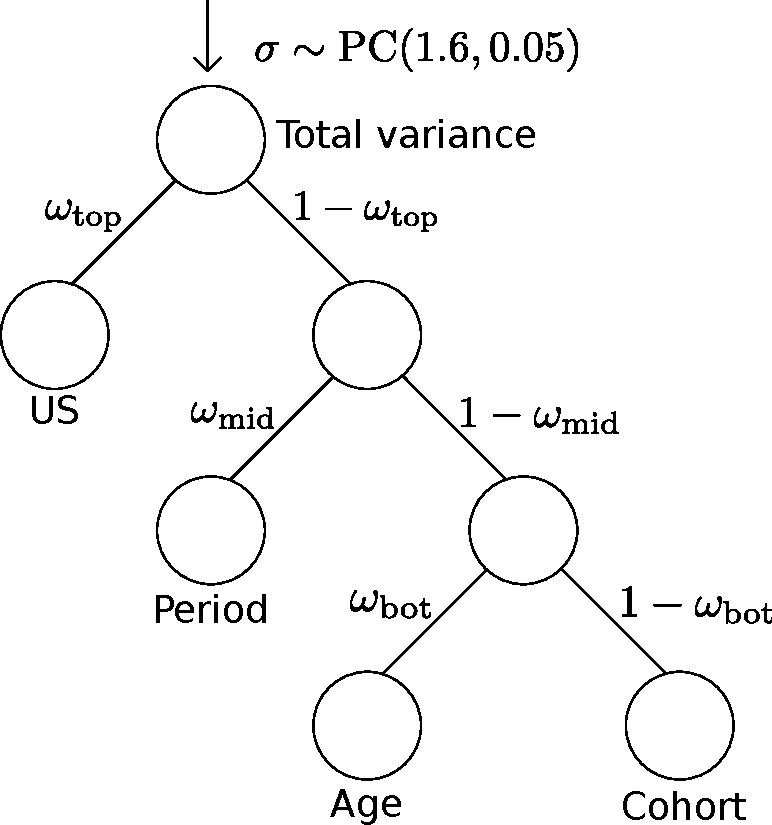
\includegraphics[width=0.6\textwidth]{Figures/Tree_some_annot.pdf}
    \caption{The hierarchical structure of the EK prior defined in Section \ref{section:application1:priorspecification}, visualized as a tree. The total variance, $\sigma^2$, is attributed to the top node, and then distributed to the unstructured (US), age, period, and cohort effects using the weight parameters $\omega_{\text{top}}$, $\omega_{\text{mid}}$, and $\omega_{\text{bot}}$ along the tree.}
    \label{figure:EK-tree}
\end{figure}

\subsubsubsection*{Alternative priors}
Naturally, a different expert on the field may disagree with the given expert knowledge. Therefore, the prior sensitivity of the model will be investigated to see how different priors affect the model. Since expert knowledge is available, an opposite or contradictory prior may be specified by doing the opposite of what is suggested by the expert knowledge. As we wish to compare the effects of different priors, preserving the same hierarchical structure is beneficial since we keep the same parameterization as the EK prior, and can compare the posteriors of $\omega_{\text{top}}$, $\omega_{\text{mid}}$ and $\omega_{\text{bot}}$. To create the "anti" prior to the EK prior while preserving the same structure, we simply swap the parameter specifying the median of the weight parameters at each split. That is, if the EK prior dictates a split attributing $30\%$ to one effect and $70\%$ to the other, this new prior then dictates that the first effect is attributed $70\%$ and the other $30\%$. The concentration parameter at each split is kept the same at $0.5$ to allow the same degree of uncertainty in the chosen median as in the EK prior. In addition, since the EK prior discourages overfitting to the structured effects by inducing shrinkage towards the unstructured effect, this new prior should induce shrinkage towards the structured effects. This "anti" prior will be dubbed the anti-EK prior.

In addition to the anti-EK prior, we may construct a prior that is unassuming in the hierarchical structure of the weight parameters. This is accomplished by attributing the total variance to the random effects using a single split with a Dirichlet(4) prior on the weight parameters. This way, the effects are considered equally important and have no enforced hierarchical structure outside the first split. The prior will simply be named the Dirichlet prior in the upcoming sections. Since the EK did not provide any information on the prior distribution of the standard deviation $\sigma$, it is kept identical as a $\text{PC}(1.6, 0.05)$ prior in all prior specifications. To bridge the gap in between the fully structured and unassuming prior structures, a prior structure with a split into structured and unstructured components was also tested, which uses a Dirichlet prior among the structured components. However, the prior structure was omitted since it achieved similar results as the other priors.

\subsubsection{Implementation in \texttt{R}}
\label{section:application1:prior-mmp}
The priors specified in Section \ref{section:application1:priorspecification} were implemented in \texttt{R} using the \texttt{makemyprior} package \citep{MMPPackage, MMP}. Details on the implementation and integration with \texttt{INLA} is found in Appendix \ref{appendix:implementation:prior}. The prior tree structure of the EK, anti-EK, and Dirichlet priors, visualized in the style of the graphical user interface in \texttt{makemyprior}, are shown in Figures \ref{figure:application1:EK}, \ref{figure:application1:antiEK}, and \ref{figure:application1:tree_dir}, respectively. In these visualizations, the width of the arrows, along with the color intensity of the nodes, represent the prior weights given to the nodes, with higher intensity and width corresponding to higher weight. The arrow width is relative to each split, which reflects the weight attribution of the split, while the color intensity shows how much of the total variance is attributed to the effect. The dashed arrows indicate shrinkage away from the node being pointed to, reflecting the shrinkages discussed in Section \ref{section:application1:priorspecification}. The prior on the total standard deviation $\sigma$ for all prior specifications is shown in Figure \ref{figure:Application1:prior_var}. The priors on the weight parameters $\omega_{\text{top}}$, $\omega_{\text{mid}}$ and $\omega_{\text{bot}}$ are shown in Figures \ref{figure:application1:dir4}, \ref{figure:application1:priors_ek}, and  \ref{figure:application1:priors_anti_ek} for the Dirichlet, EK and, anti-EK priors, respectively. 

\captionsetup[subfigure]{labelfont={bf,large}, font={large}, skip=1pt, margin=0cm, singlelinecheck=true}
%MMP EK and anti-EK structure 
\begin{figure}[h!]
    \centering
    \begin{subfigure}[b]{0.470\textwidth}   
        \centering 
        %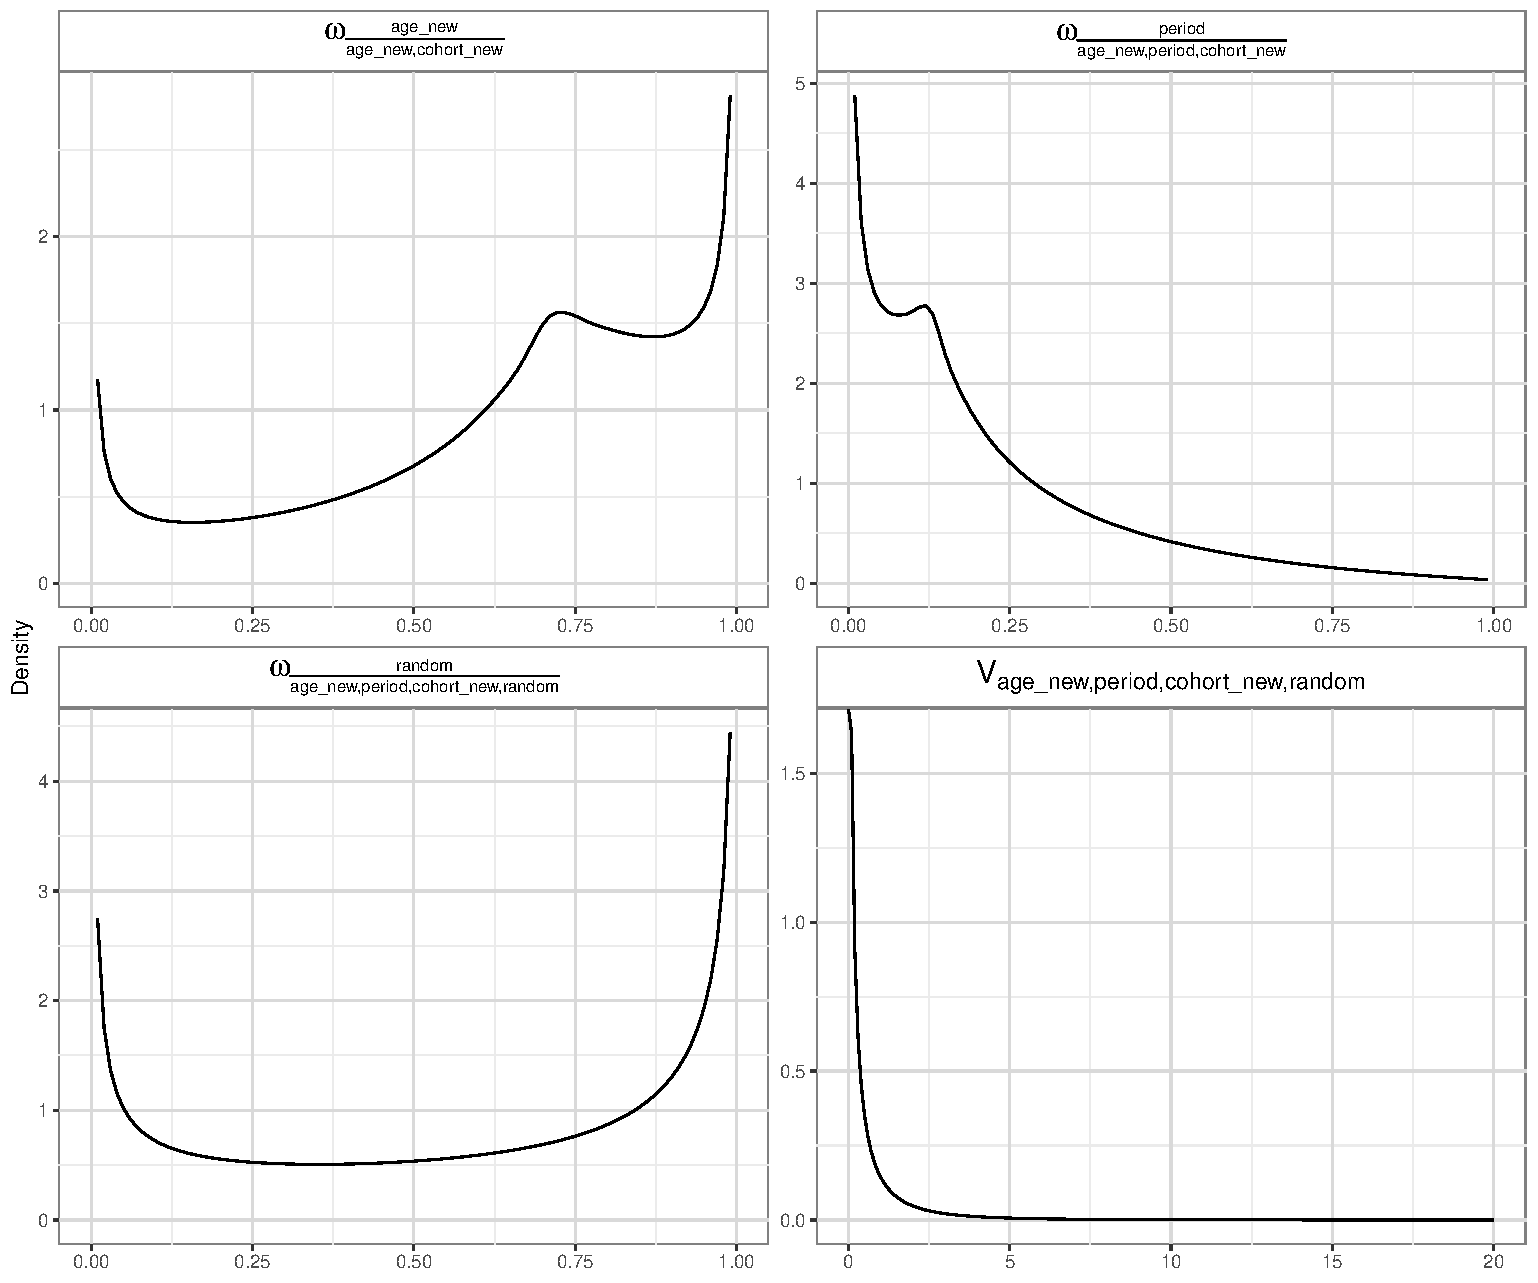
\includegraphics[width=\textwidth]{Figures/Prior_expert.png}
        
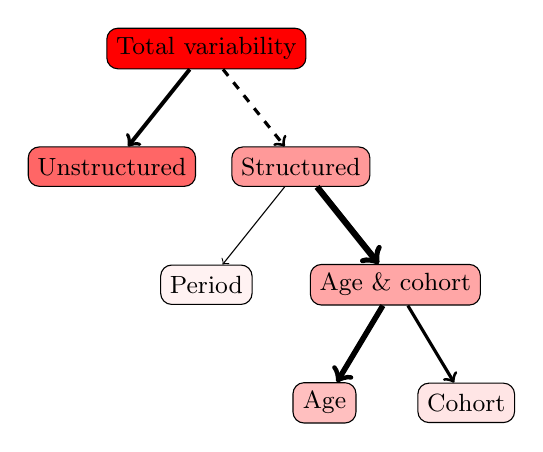
\begin{tikzpicture}[
    rounded corners,
    minimum height = 0.5cm, 
    minimum width = 0.8cm
]
\node[draw] (top) [fill = red!100] {{\color{black}\small Total variability}};
\node[draw] (gen) [below of = top, xshift = 1.2cm, yshift = -0.5cm, fill = red!40] {\small Structured};
\node[draw] (env) [below of = top, xshift = -1.2cm, yshift = -0.5cm, fill = red!60] {\small Unstructured};
\node[draw] (add) [below of = gen, xshift = -1.2cm, yshift = -0.5cm, fill = red!5] {\small Period};
\node[draw] (nonadd) [below of = gen, xshift = 1.2cm, yshift = -0.5cm, fill = red!35] {\small Age \& cohort};
\node[draw] (dom) [below of = nonadd, xshift = -0.9cm, yshift = -0.5cm, fill = red!25] {\small Age};
\node[draw] (epi) [below of = nonadd, xshift = 0.9cm, yshift = -0.5cm, fill = red!10] {\small Cohort};
% arrows
\path[->, every node/.style = {sloped, anchor = south, auto = false, anchor = mid, yshift = 0.15cm}]
(top) edge[line width = 0.5mm] node[] {} (env)
(top) edge[dashed, line width = 0.4mm] node[] {} (gen)
(gen) edge[] node[] {} (add)
(gen) edge[line width = 0.8mm] node[] {} (nonadd)
(nonadd) edge[line width = 0.7mm] node[] {} (dom)
(nonadd) edge[line width = 0.4mm] node[] {} (epi);

\end{tikzpicture}

        \caption[]%
        {{\small EK prior}}    
        \label{figure:application1:EK}
    \end{subfigure}
    \hfill
    \begin{subfigure}[b]{0.470\textwidth}   
        \centering 
        %\includegraphics[width=\textwidth]{Figures/Prior_anti.png}
        
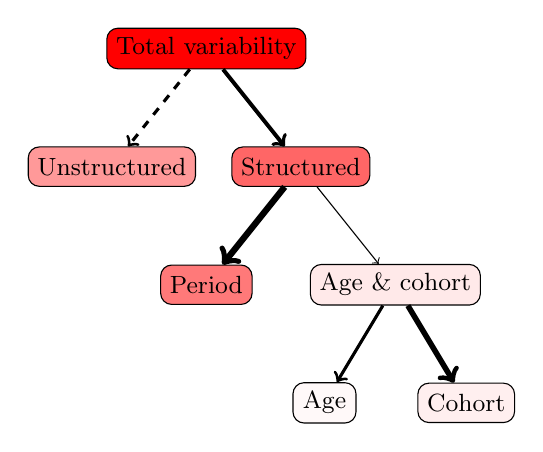
\begin{tikzpicture}[
    rounded corners,
    minimum height = 0.5cm, 
    minimum width = 0.8cm
]
\node[draw] (top) [fill = red!100] {{\color{black}\small Total variability}};
\node[draw] (gen) [below of = top, xshift = 1.2cm, yshift = -0.5cm, fill = red!60] {\small Structured};
\node[draw] (env) [below of = top, xshift = -1.2cm, yshift = -0.5cm, fill = red!40] {\small Unstructured};
\node[draw] (add) [below of = gen, xshift = -1.2cm, yshift = -0.5cm, fill = red!52.5] {\small Period};
\node[draw] (nonadd) [below of = gen, xshift = 1.2cm, yshift = -0.5cm, fill = red!8.5] {\small Age \& cohort};
\node[draw] (dom) [below of = nonadd, xshift = -0.9cm, yshift = -0.5cm, fill = red!2.4] {\small Age};
\node[draw] (epi) [below of = nonadd, xshift = 0.9cm, yshift = -0.5cm, fill = red!6.1] {\small Cohort};
% arrows
\path[->, every node/.style = {sloped, anchor = south, auto = false, anchor = mid, yshift = 0.15cm}]
(top) edge[dashed, line width = 0.4mm] node[] {} (env)
(top) edge[line width = 0.5mm] node[] {} (gen)
(gen) edge[line width = 0.8mm] node[] {} (add)
(gen) edge[] node[] {} (nonadd)
(nonadd) edge[line width = 0.4mm] node[] {} (dom)
(nonadd) edge[line width = 0.7mm] node[] {} (epi);

\end{tikzpicture}

        \caption[]%
        {{\small Anti-EK prior}}    
        \label{figure:application1:antiEK}
    \end{subfigure}
    \caption{Visualization of the attribution of variance in the \textbf{(a)} EK prior and \textbf{(b)} anti-EK prior defined in Section \ref{section:application1:priorspecification}. Greater arrow width corresponds to higher weight attribution in the split, and the dashed arrow indicates shrinkage away from the effect. The color intensity of the nodes correspond to the proportion of the total variance attributed to the effect.}
    \label{fig:result:prior}
\end{figure}

%MMP prior plots
\begin{figure}[h!]
    \centering
    \begin{subfigure}[b]{0.9\textwidth}
        \centering
        %\includegraphics[width=\textwidth]{Figures/Prior_dir.png}
        
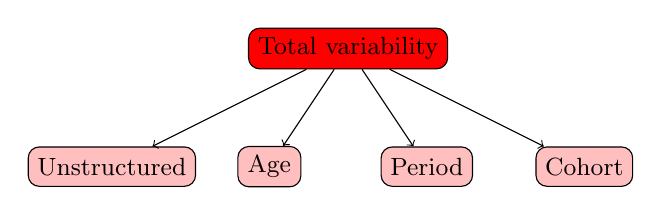
\begin{tikzpicture}[
    rounded corners,
    minimum height = 0.5cm, 
    minimum width = 0.8cm
]
\node[draw] (top) [fill = red!100] {{\color{black}\small Total variability}};
\node[draw] (US) [below of = top, xshift = -3cm, yshift = -0.5cm, fill = red!25] {\small Unstructured};
\node[draw] (Age) [below of = top, xshift = -1cm, yshift = -0.5cm, fill = red!25] {\small Age};
\node[draw] (Period) [below of = top, xshift = 1cm, yshift = -0.5cm, fill = red!25] {\small Period};
\node[draw] (Cohort) [below of = top, xshift = 3cm, yshift = -0.5cm, fill = red!25] {\small Cohort};
% arrows
\path[->, every node/.style = {sloped, anchor = south, auto = false, anchor = mid, yshift = 0.15cm}]
(top) edge[] node[] {} (US)
(top) edge[] node[] {} (Age)
(top) edge[] node[] {} (Period)
(top) edge[] node[] {} (Cohort)
;

\end{tikzpicture}

        \vspace{0.2cm}
        \caption[]{{\small Prior tree structure}}    
        \label{figure:application1:tree_dir}
    \end{subfigure}
    \vskip\baselineskip\vspace{-0.3cm}
    \begin{subfigure}[b]{0.35\textwidth}   
        \centering 
        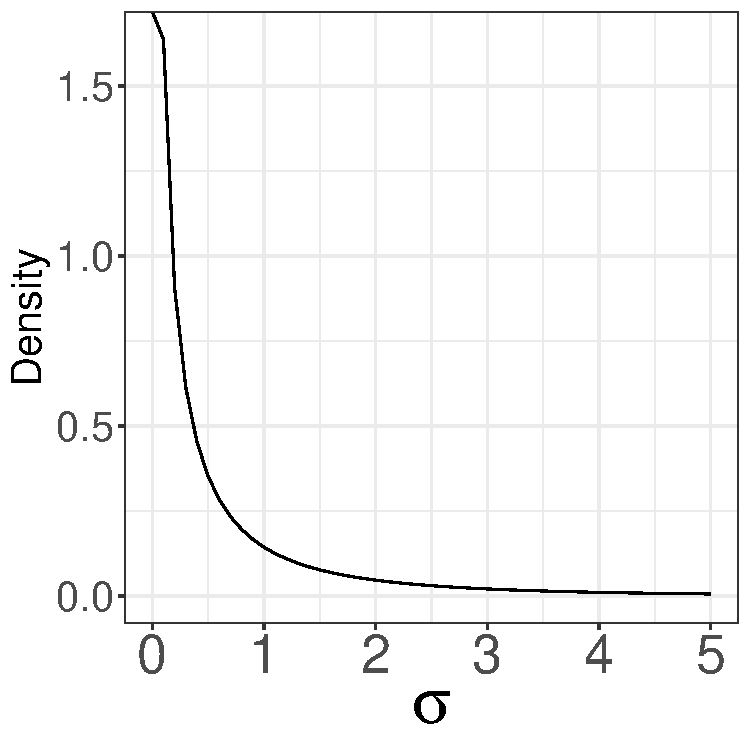
\includegraphics[width=\linewidth]{./Figures/prior_V.pdf}
        \caption[]{\small{$\text{PC}(1.6,0.05)$}}
        \label{figure:Application1:prior_var}
    \end{subfigure}
    \hspace{1cm}
    \begin{subfigure}[b]{0.35\textwidth}   
        \centering 
        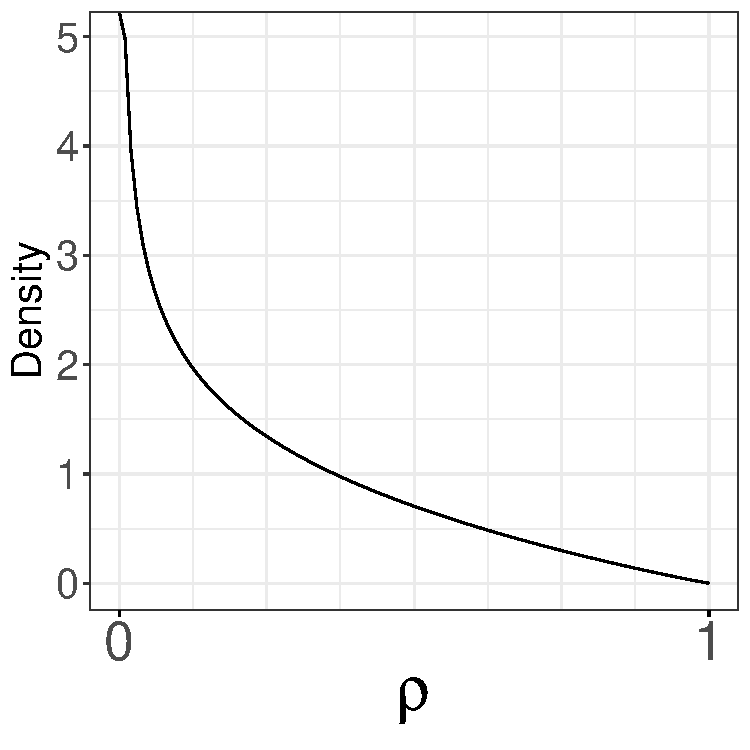
\includegraphics[width=\textwidth]{Figures/prior_dir4.pdf}
        \caption[]%
        {{\small Dirichlet(4)}}    
        \label{figure:application1:dir4}
    \end{subfigure}
    \caption{\textbf{(a)} The attribution of the total variance to the unstructured, age, period and cohort effects in the Dirichlet prior defined in Section \ref{section:application1:priorspecification}. The equal color intensity of the nodes and uniform arrow width highlight the equal proportion of the total variance attributed to each effect. \textbf{(b)} Single weight parameter of a Dirichlet$(4)$ prior distribution. \textbf{(c)} The $\text{PC}(1.6,0.05)$ prior placed on the standard deviation in all prior structures specified in Section \ref{section:application1:priorspecification}. }
    \label{fig:application1:priors}
\end{figure}

%Prior of ek
\begin{figure}[h!]
    \centering
    \begin{subfigure}[b]{0.99\textwidth}
        \centering
        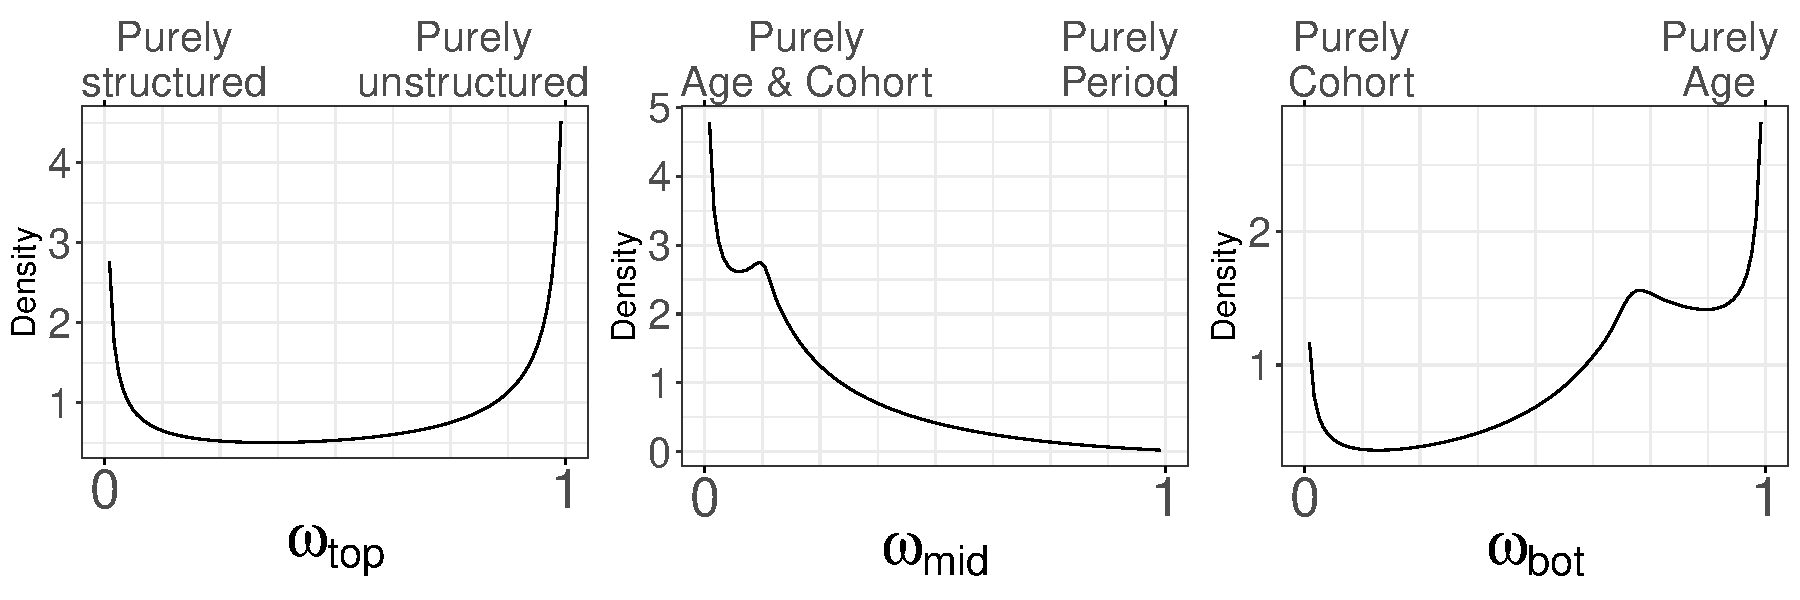
\includegraphics[width=\textwidth]{Figures/prior_rest.pdf}
        \caption[Network2]%
        {{\small EK prior}}    
        \label{figure:application1:priors_ek}
    \end{subfigure}
    \vskip\baselineskip\vspace{-0.5cm}
    \begin{subfigure}[b]{0.99\textwidth}   
        \centering 
        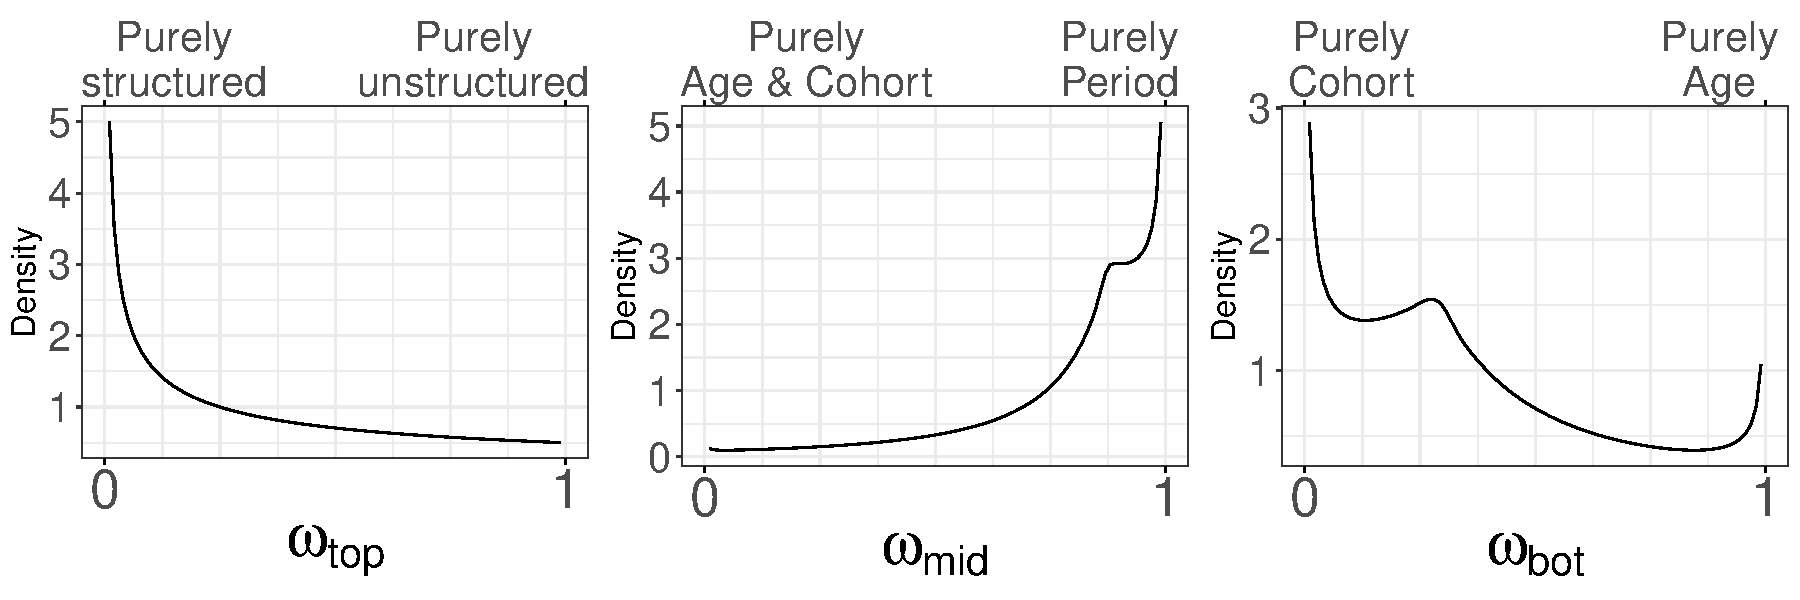
\includegraphics[width=\textwidth]{Figures/prior_rest_anti.pdf}
        \caption[]%
        {{\small Anti-EK prior}}    
        \label{figure:application1:priors_anti_ek}
    \end{subfigure}
    \caption{The prior distributions placed on the weight parameters $\omega_{\text{top}}$, $\omega_{\text{mid}}$, and $\omega_{\text{bot}}$ in \textbf{(a)} the EK prior and \textbf{(b)} the anti-EK prior, as defined in Section \ref{section:application1:priorspecification}. The location of the weight parameters along the prior tree structure is illustrated in Figure \ref{figure:EK-tree} with the same names, giving rise to the visualization in Figure \ref{fig:result:prior}.}
    \label{figure:application1:priors_weights}
\end{figure}


\FloatBarrier
\subsection{Posterior inference}
\label{section:application1:posteriorInference}
As mentioned in Sections \ref{section:Introduction} and \ref{section:Age-period-cohort-models}, a major consideration when using MAPC models is the issue of identifiability of the temporal effects. The random effects themselves are not identifiable due to their implicit linear dependence, but the linear predictor is identifiable, meaning we can use differences of the linear predictor to infer around the effect of stratification by educational attainment. In Section \ref{section:data:explorative}, we argued that BA+ level of attained education should serve as the baseline level for comparison. Using the definitions of the cross strata differences in Section \ref{section:APC-inference}, this corresponds to selecting BA+ to denote stratum $r_1$ in Equations \eqref{eqn:deltajk} and \eqref{eqn:deltak}. Moreover, in the presence of only one stratum-specific effect, we recall that when applying the exponential function to the cross strata differences, we interpret it as a ratio of odds. Should two stratum-specific effects be present, the interpretation changes to being the geometric mean of the odds ratio with respect to one temporal index, where the geometric mean is taken over the other temporal index. In practice, we do not compute the averaged differences which we interpret as the log-odds ratios, but rather define linear combinations of the stratum-specific intercepts and effects to be computed. By our Bayesian framework, each effect is now considered to be Gaussian a priori, meaning that our odds ratios also are considered Gaussian. Consequently, we may derive $95\%$ credible intervals in our inference. As for our given estimates, we will be using the median.  

The computation of these cross strata differences is easily performed in \texttt{INLA} by predefining linear combinations of the effects over the temporal indices to be computed using \texttt{inla.make.lincomb()}. An example of how these are provided is shown in Appendix \ref{appendix:implementation:lincombs}.

\FloatBarrier
\subsection{Model selection}
\label{section:model-selection}
With our methods and implementations in order, the only task left for a complete model specification is to complete the model choice by determining which effects should be shared between the different strata, and which effects should be stratum-specific. As mentioned in Section \ref{section:application1:priorspecification}, a requirement for the identifiability of the cross strata differences is that there is at least one shared effect and at least one stratum-specific effect. As a consequence of these requirements, we have $6$ candidate models from which we wish to select the one with the best fit. To rank the models, we use the logarithmic score, as well as WAIC and DIC (all described in Appendix \ref{section:disease-mapping:criteria}). All models are fitted using the EK prior.

\begin{table}[h!]
\centering
\begingroup\footnotesize\setstretch{1.2}

\begin{tabularx}{\textwidth}{llXXXXXX}
\hline
 &  & apC & aPc & aPC & Apc & ApC & \multicolumn{1}{c}{APc} \\ 
\hline
\nopagebreak log-score & \nopagebreak Female  & 2.673 & \textbf{ 2.669 } & 2.674 & 2.677 & 2.697 & 2.677 \\
 & \nopagebreak Male  & 2.500 & \textbf{ 2.497 } & 2.500 & 2.502 & 2.513 & 2.500 \\
\rule{0pt}{0.9\normalbaselineskip}WAIC & \nopagebreak Female  & 28228 & \textbf{ 28182 } & 28236 & 28270 & 28474 & 28265 \\
 & \nopagebreak Male  & 26394 & \textbf{ 26369 } & 26394 & 26417 & 26529 & 26403 \\
\rule{0pt}{0.9\normalbaselineskip}DIC & \nopagebreak Female  & 28221 & \textbf{ 28179 } & 28230 & 28263 & 28460 & 28259 \\
 & \nopagebreak Male  & 26392 & \textbf{ 26367 } & 26390 & 26411 & 26522 & 26400 \\
\hline 
\end{tabularx}\endgroup
 \caption{The achieved logarithmic score, WAIC, and DIC for each of the 6 candidate MAPC models, specified by different combinations of stratum-specific and shared age, period, and cohort effects. Shared effects are denoted with uppercase letters, and stratum-specific effects are denoted with lowercase letters. For each sex, the best model by each criterion is highlighted in bold.} \label{fig:model_selection_score}


\end{table}

The computed logarithmic score, WAIC, and DIC are shown in Table \ref{fig:model_selection_score} for all possible configurations of shared and stratum-specific effects, with the best models highlighted in bold for both sexes. Overall, the computed logarithmic scores, WAIC, and DIC are very similar within the male and female groups. The aPc model achieved the lowest logarithmic score for both sexes, and will therefore be interpreted in detail in the upcoming Section. From the lowest to highest scores, excluding the aPc model, are the apC, aPC, APc, Apc and ApC models. The scores of the top four models are very similar, and it would therefore be interesting to investigate the differences between these models.

\FloatBarrier
\subsection{Prior sensitivity analysis}
\label{section:application1:prior-sens}
\subsubsection{Methods}
\label{section:application1:prior-sens-motiv}
As this is a Bayesian analysis, we wish to carry out a prior sensitivity analysis using the EK, anti-EK, Dirichlet, and component-specific priors defined back in Section \ref{section:application1:priorspecification}. In addition, we investigate how models using joint prior specifications compare to models using component-specific priors, which is done by including a component-specific prior chosen unsubjectively as yet another contrast to the subjective prior elicited from EK.

We compare the effects of the priors on the model by comparing the posterior distributions of the estimated standard deviation $\sigma$, along with the weight parameters $\omega_{\text{top}}$, $\omega_{\text{mid}}$, and $\omega_{\text{bot}}$. Due to the different hierarchical structures of the Dirichlet and component-specific priors compared to the EK and anti-EK prior, direct and formal comparisons of the posteriors is difficult. Since we wish to compare the posteriors with respect to the EK prior, we estimate the posterior distributions of the weight parameters for the other priors at the levels of the EK prior. This also applies to the component-specific prior we also want to compare with. To remedy the issue of different structures, we sample the precision parameters from the posterior distributions and then transform them to match the levels of the hierarchical structure of the EK prior by Equations \eqref{eqn:omega_def}. While this does not reflect the structure of the used prior, it still allows for qualitative comparison to the EK prior, meaning we will be able to see if the different priors cause a different interpretation of the resulting model.

\FloatBarrier
\subsubsection{Results}
\label{section:application1:prior-sens-result}
Figures \ref{figure:Application1:s0_f}, \ref{figure:Application1:s1_f}, \ref{figure:Application1:s2_f}, and \ref{figure:Application1:s3_f} show the prior and posterior distributions of the standard deviation and mixing parameters which are on the levels presented in the hierarchical decomposition prior tree in Figure \ref{figure:EK-tree} for the aPc model using data on female participants. To obtain the posterior distributions, 10,000 samples of the hyperparameters of each model were used. For the observed variance, shown in Figure \ref{figure:Application1:s0_f}, we observe that the posteriors are very similar despite the different prior specifications. In particular, it is interesting to note that the posterior using component-specific (CS) priors is also similar to the other models despite not sharing an identical prior at this level. On the first split of the tree, we see in Figure \ref{figure:Application1:s1_f} that the posterior places nearly all the weight of the mixing parameters on the temporally-structured components, and very little on the unstructured random effect. This is particularly interesting in the case of the model using EK, since this model facilitated shrinkage toward the unstructured random effect. Despite the shrinkage, the model clearly favors the structured components. In Figure \ref{figure:Application1:s2_f}, we also see that the different priors produce quite similar posteriors though with some slight differences. Here, the weight parameter clearly favors the age and cohort effects, i.e., the education-specific effects. For the last split, we once again see similar posteriors in Figure \ref{figure:Application1:s3_f}, with only small differences in the median estimate. Here we see that the median estimates are close to $0.5$, showing a preference to balance the education-specific effects. Overall, we see that the posterior distributions are very similar to each other, despite the use of very different priors. The equivalent plots using data on male participants is shown in Appendix \ref{appendix:figures} in Figures \ref{figure:Application1:s0_m} and \ref{figure:Application1:compare-plots_m}, and they exhibit the same behaviors as for the female data. In conclusion, the data is very informative, and therefore the models are not very sensitive to the prior.

\begin{figure}[!ht]
    \centering
    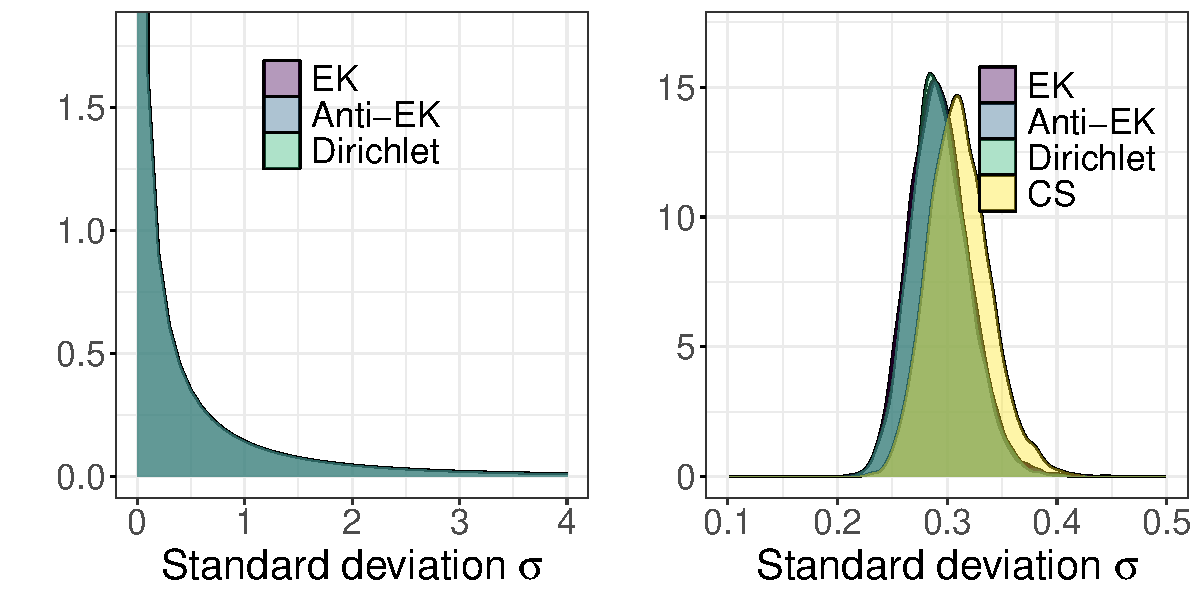
\includegraphics[width=0.8\textwidth]{Figures/compare_plots_s0_f.pdf}
    \caption{The (left) prior and (right) posterior distributions of the standard deviation in aPc models using female data along with the expert knowledge (EK), anti-EK, Dirichlet, and component-specific (CS) priors outlined in Section \ref{section:application1:prior}. }
    \label{figure:Application1:s0_f}
\end{figure}

\begin{figure}[!ht]
    \centering
    \begin{subfigure}[b]{0.8\textwidth}
        \centering
        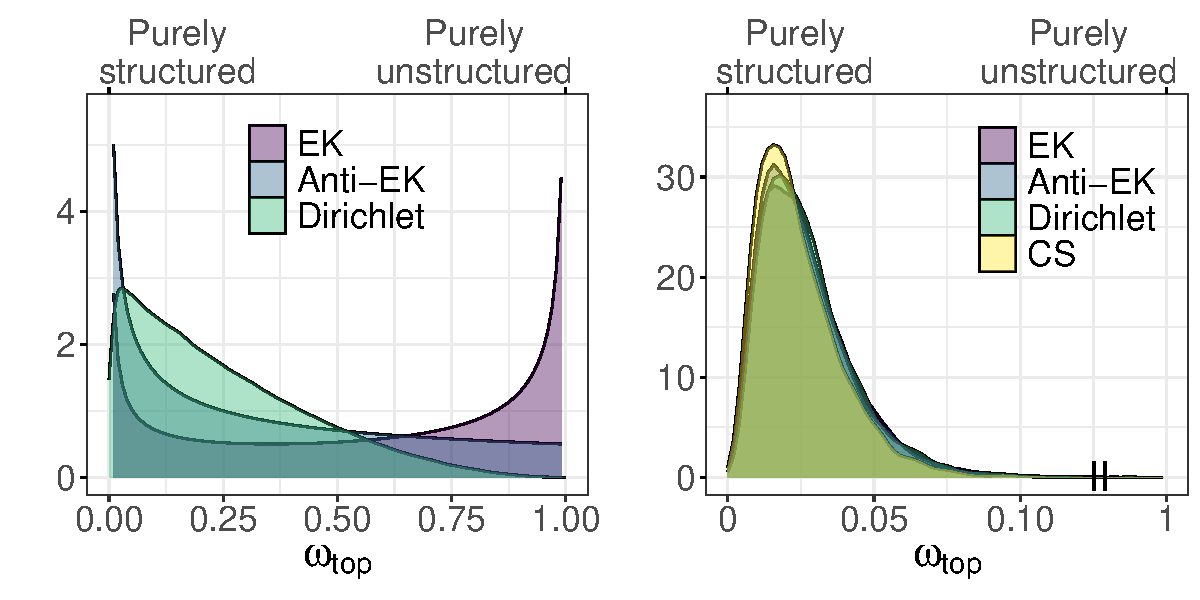
\includegraphics[width=\textwidth]{Figures/compare_plots_s1_f.pdf}
        \caption[Network2]%
        {{\small Top split}}    
        \label{figure:Application1:s1_f}
    \end{subfigure}
    \vskip\baselineskip\vspace{-0.5cm}
    \begin{subfigure}[b]{0.8\textwidth}   
        \centering 
        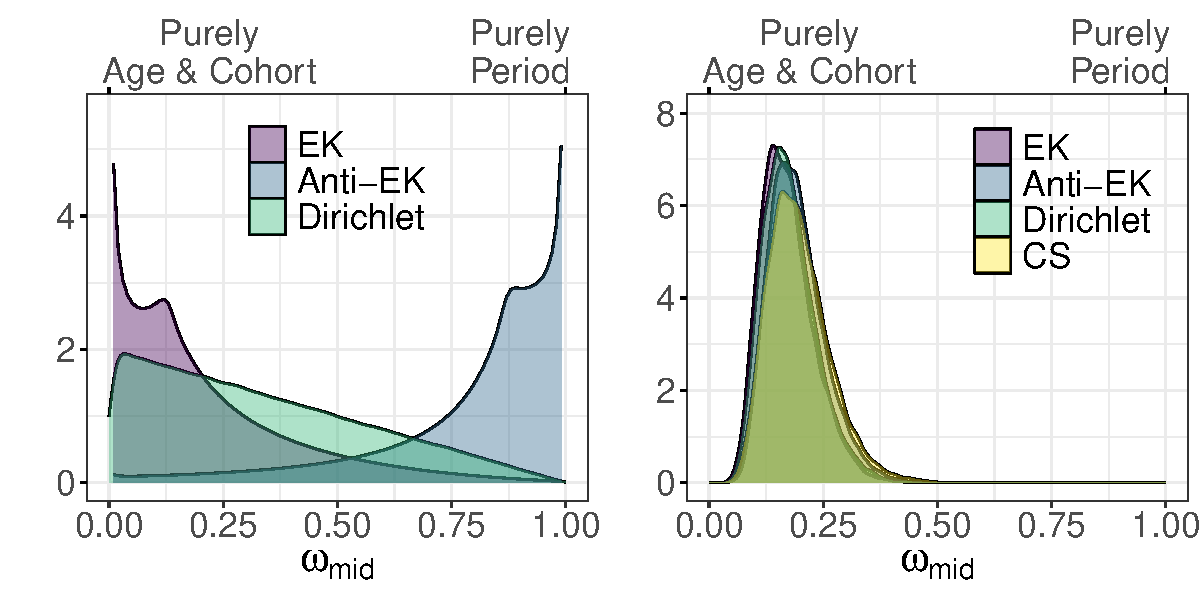
\includegraphics[width=\textwidth]{Figures/compare_plots_s2_f.pdf}
        \caption[]%
        {{\small Middle split}}    
        \label{figure:Application1:s2_f}
    \end{subfigure}
    \vskip\baselineskip\vspace{-0.5cm}
    \begin{subfigure}[b]{0.8\textwidth}   
        \centering 
        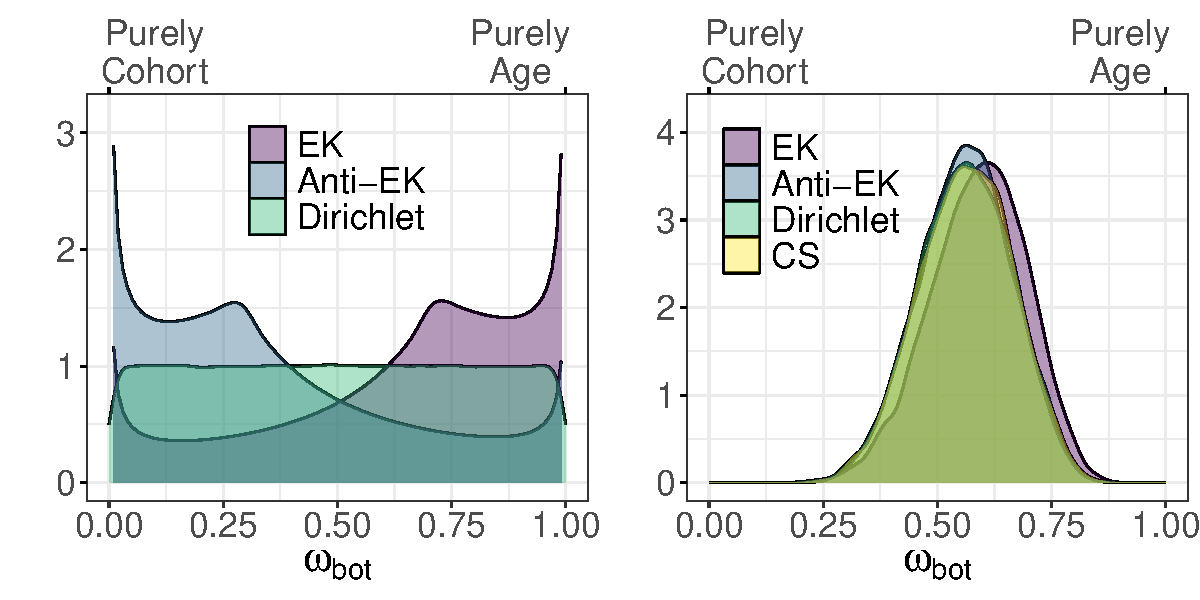
\includegraphics[width=\textwidth]{Figures/compare_plots_s3_f.pdf}
        \caption[]%
        {{\small  Bottom split}}    
        \label{figure:Application1:s3_f}
    \end{subfigure}
    \vspace{-0.2cm}
    \caption{The (left) prior and (right) posterior distribution of the mixing parameters at the \textbf{(a)} top, \textbf{(b)} middle, and \textbf{(c)} bottom levels in the hierarchical structure of the EK prior in aPc models using female data and the expert knowledge (EK), anti-EK, Dirichlet, and component-specific (CS) priors outlined in Section \ref{section:application1:prior}. }
    \label{fig:application1:compare-plots_f}
\end{figure}

\FloatBarrier
\subsection{Results}\label{section:application1:results}
\subsubsubsection*{Summary}
\vspace{-0.2cm}
For different levels of attained education, Figure \ref{figure:Application1:lincombs_best} shows the posterior medians of the odds ratio, as described in Section \ref{section:APC-inference}, over the relevant temporal indices in the aPc model using the EK prior for females and males separately, along with $95\%$ credible intervals. As these models incorporate education-specific age and cohort effects, the odds ratios over these two temporal indices are presented. As discussed in Section \ref{section:APC-inference}, the estimated odds ratios are with respect to the highest level of attained education, BA+. An odds ratio of $2$ implies that the odds are twice as large as in the group we compare with (BA+, in this case). A key observation is that in all figures, the estimated odds ratios are greater than $1$ everywhere, with credible intervals rarely including this value. By our discussion on the odds ratio in Section \ref{section:APC-inference}, this indicates a greater risk of back pain in all age groups and cohorts compared to BA+.

\captionsetup[subfigure]{font={bf,large}, skip=1pt, margin=0cm, singlelinecheck=false}

%Best model both sexes
\begin{figure}[h!]
    \centering
    \begin{subfigure}[b]{\textwidth}   
        \centering 
        \caption[]%
        {}    
        \label{figure:Application1:best_age_diff}
        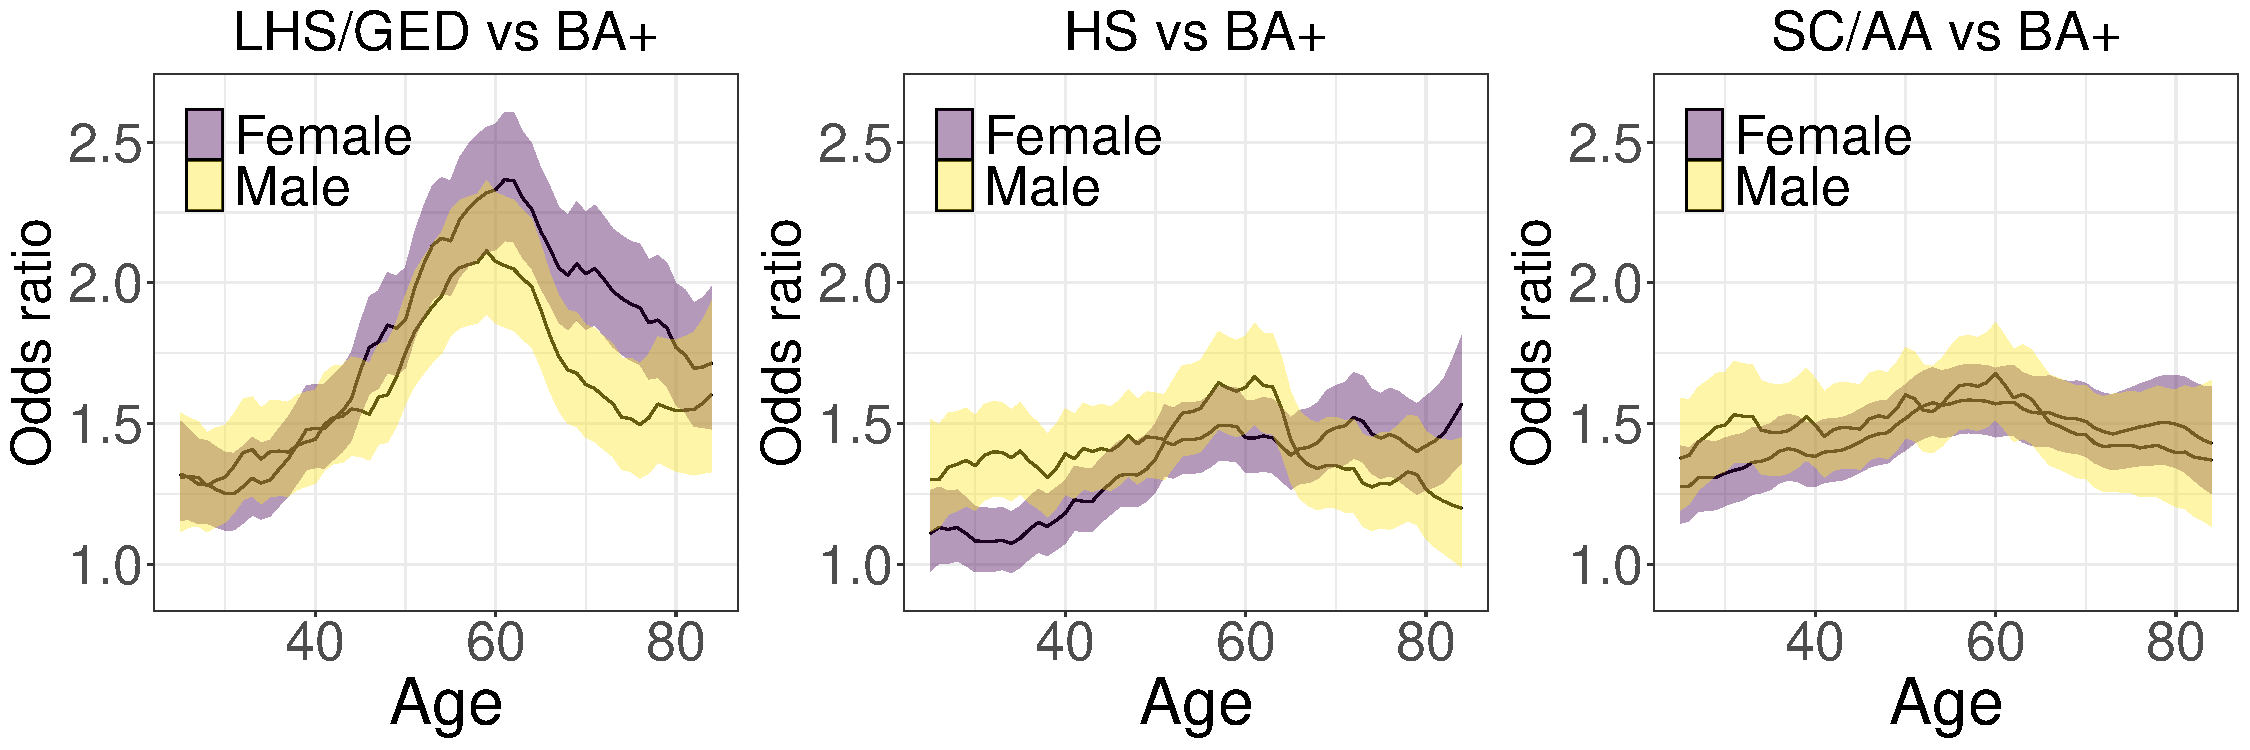
\includegraphics[width=\textwidth]{Figures/best_lincomb_age.pdf}
    \end{subfigure}
    \vskip\baselineskip\vspace{-0.3cm}
    \begin{subfigure}[b]{\textwidth}   
        \centering 
        \caption[]%
        {}    
        \label{figure:Application1:best_cohort_diff}
        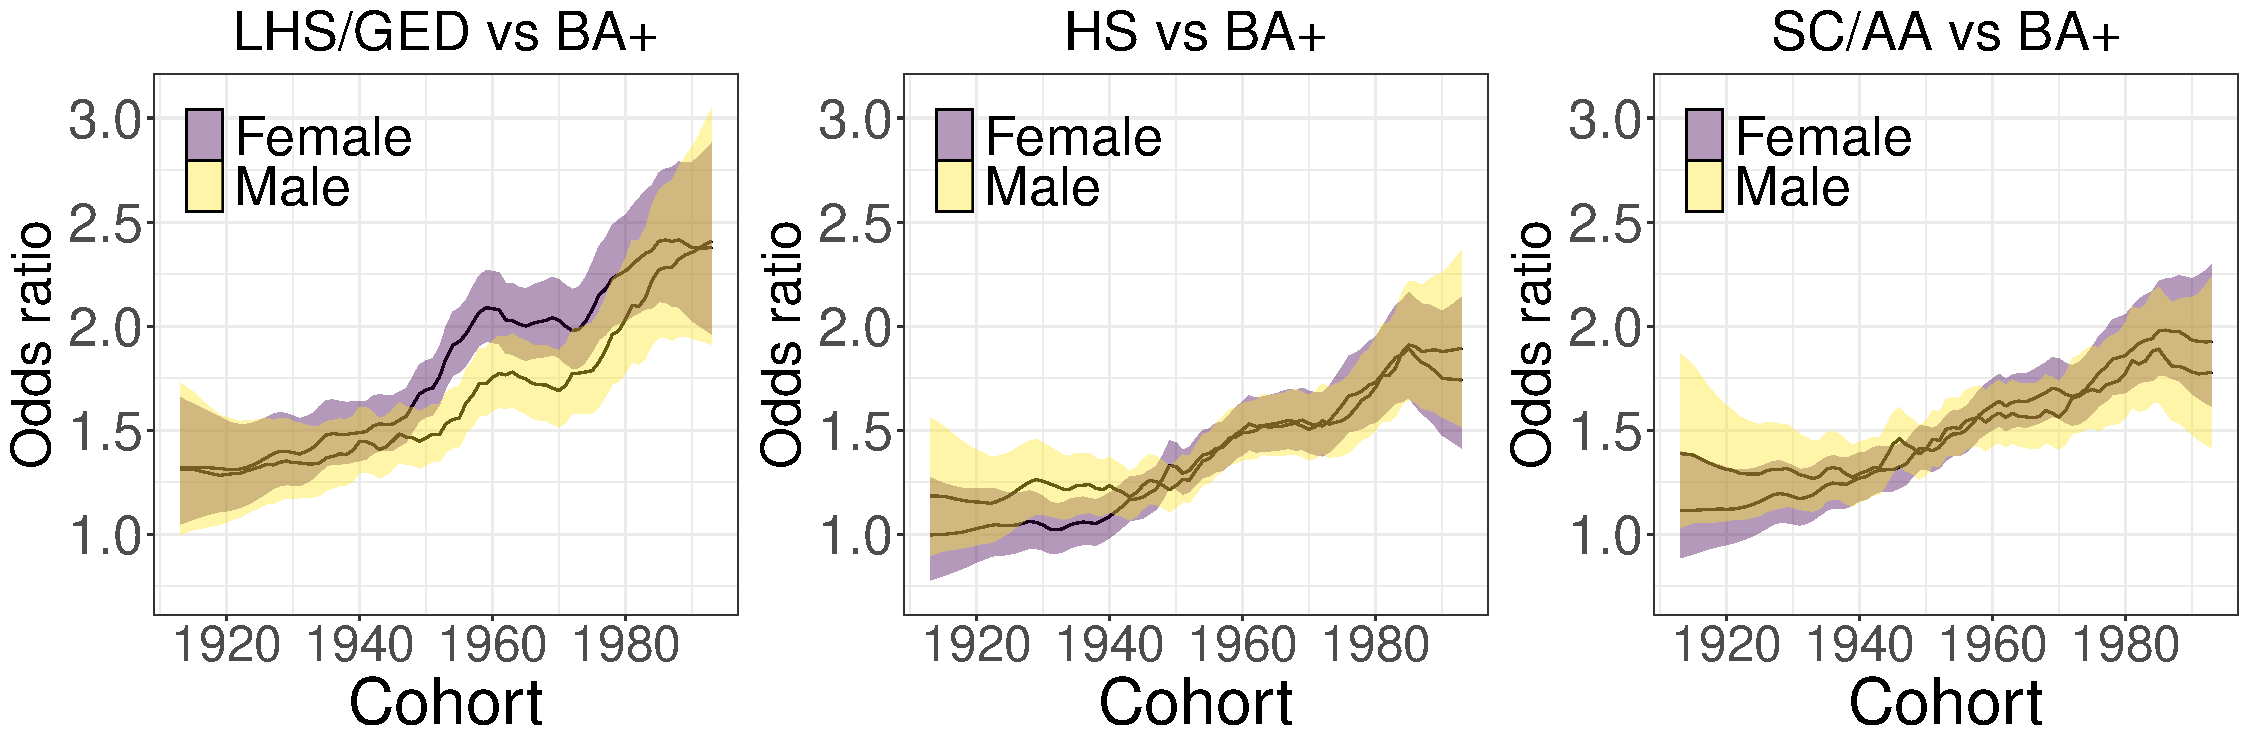
\includegraphics[width=\textwidth]{Figures/best_lincomb_cohort.pdf}
    \end{subfigure}
    \vspace{-0.2cm}
    \caption{Less than high school (LHS), high school (HS), and some college/associate of arts degree (SC/AA) levels of attained education with respect to bachelor or higher education (BA+), the posterior median odds ratio over \textbf{(a)} age and \textbf{(b)} cohorts, along with $95\%$ credible intervals. The trends are shown separately for males and females using the aPc model.}
    \label{figure:Application1:lincombs_best}
\end{figure}

\subsubsubsection*{Trends over age}
\vspace{-0.2cm}
In the estimated odds ratios over age, in Figure \ref{figure:Application1:best_age_diff}, we observe similar trends between males and females in the LHS/GED and SC/AA levels of attained education. Meanwhile, some dissimilarities are observed for the HS level of attained education. For the LHS/GED level of attained education, we observe estimated odds ratios of around $1.3$ for both sexes in the youngest age groups, increasing steadily to $2.1$ for males and $2.35$ for females by age $60$, before declining to $1.6$ for males and $1.75$ for females by age $84$. This rising and falling (inverse V-shape) trend is also vaguely observed for the SC/AA level of attained education, though with smaller differences between the sexes. For the SC/AA level of attained education, the odds ratios are estimated around $1.25$ for females and $1.4$ for males at age $25$, increasing somewhat linearly to around $1.6$ for both sexes by age $55$ before declining to around $1.4$ to $1.45$ by age $84$. On the other hand, in the case of HS level of attained education, the trends visibly differ between the sexes. For males, we observe a less pronounced inverse V-shape trend, starting at $1.25$ at age $25$, increasing to $1.65$ by age $60$, before declining to $1.25$ again by age $84$. For females, the trend of odds ratios begins at $1.15$ at age $25$, increasing to around $1.4$ by age $50$, and remaining at this level until age $84$. In addition, we observe a particularly high risk of back pain among participants with LHS/GED levels of attained education, with odds ratios estimated as high as $2.35$ in some age groups. It is also interesting to note that female participants with LHS/GED level of attained education are more at risk than their male counterpart in age groups above $45$, while it is more even for the two other levels of education. 

%Over cohort
\subsubsubsection*{Trends over cohorts}
\vspace{-0.2cm}
In the estimated odds ratios over cohort, in Figure \ref{figure:Application1:best_cohort_diff}, we observe similar trends for both males and females, increasing with more recent cohorts in all levels of attained education. In the LHS/GED level of attained education, we observe odds ratio estimates of around $1.25$ for both sexes in the $1913$ birth cohort, increasing to $1.75$ for males and $2.05$ for females by the $1960$ birth cohort. The estimated odds ratios remain at these levels until the $1975$ birth cohort, after which the odds ratios begin to increase significantly to around $2.4$ for both sexes by the $1993$ birth cohort. For both the HS and SC/AA levels of attained education, we observe odds ratios of $1$ for females and $1.3$ for males in the $1913$ birth cohort, steadily increasing to around $1.85$ for both sexes by the $1985$ birth cohort. The estimated odds ratios remain at this level until the $1993$ birth cohort. As with the odds ratios over age, the estimated odds ratio is greater than $1$ almost everywhere, indicating that all participants with level of attained education lower than BA+ have a greater risk of backpain compared to the corresponding cohorts with BA+ level of attained education. We also observe higher risk particularly among participants with LHS/GED level of attained education, reaching odds ratios up to $2.4$.

%Top3 models female
\begin{figure}
    \centering
    \begin{subfigure}[b]{\textwidth}   
        \centering 
        \caption[]%
        {}    
        \label{figure:Application1:age_diff_f}
        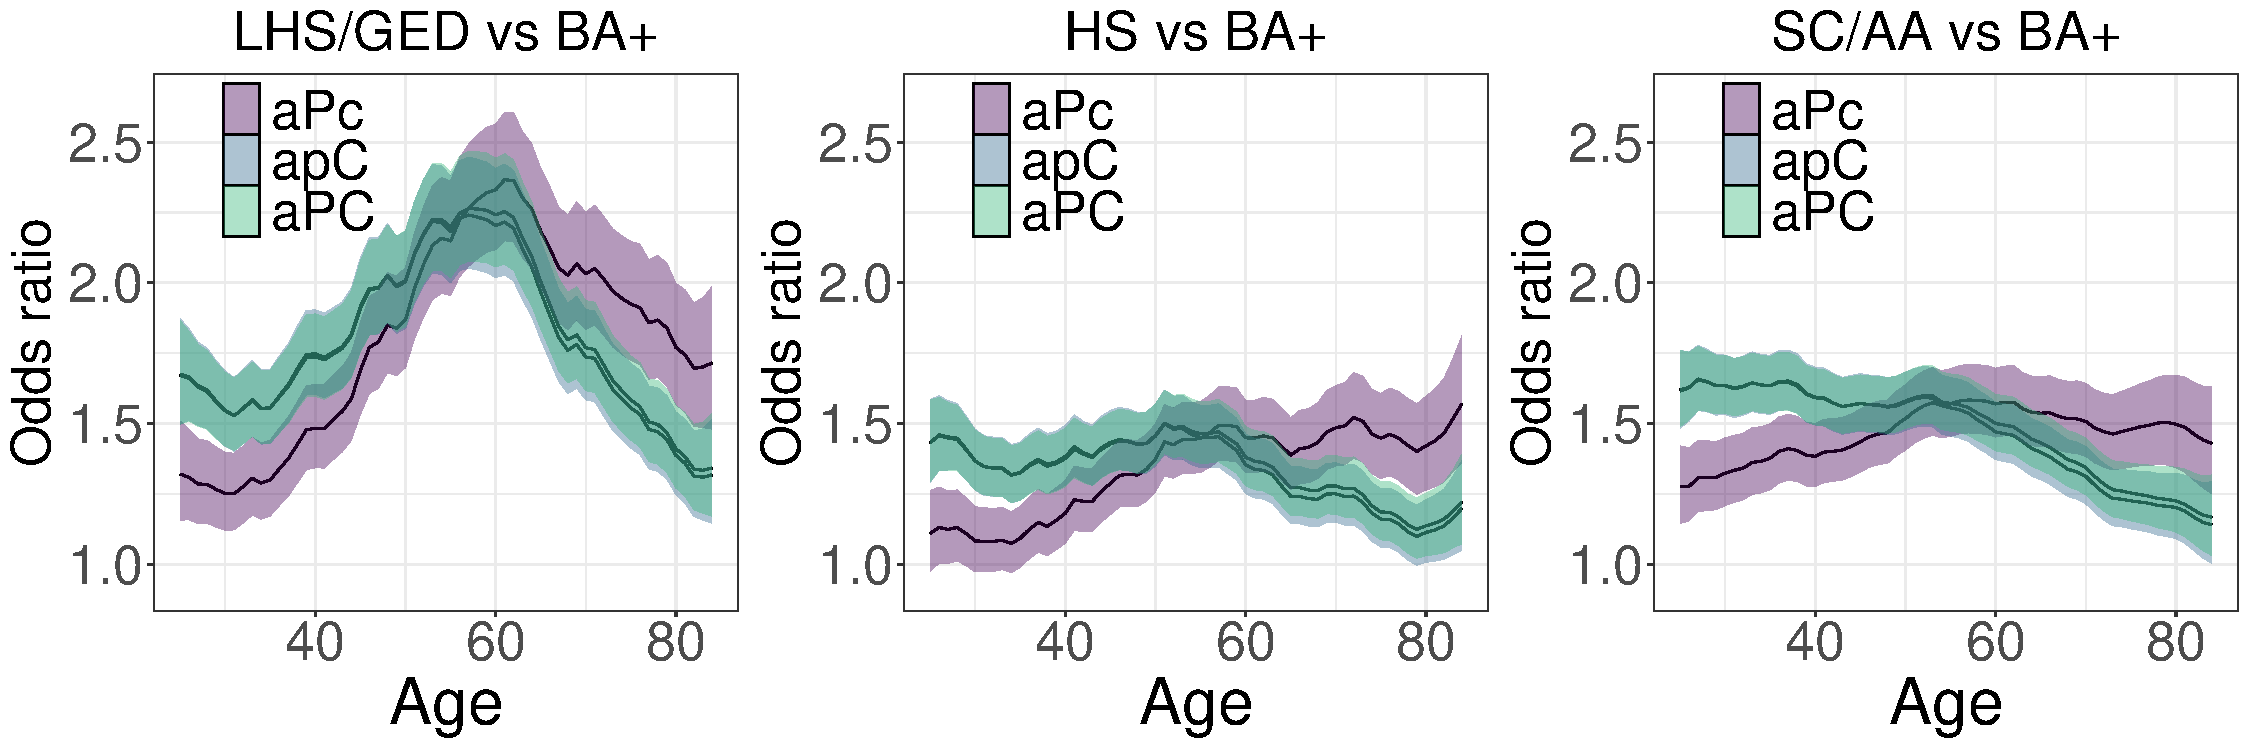
\includegraphics[width=\textwidth]{Figures/lincomb_age_f.pdf}
    \end{subfigure}
    \vskip\baselineskip\vspace{-0.3cm}
    \begin{subfigure}[b]{\textwidth}   
        \centering 
        \caption[]%
        {}    
        \label{figure:Application1:period_diff_f}
        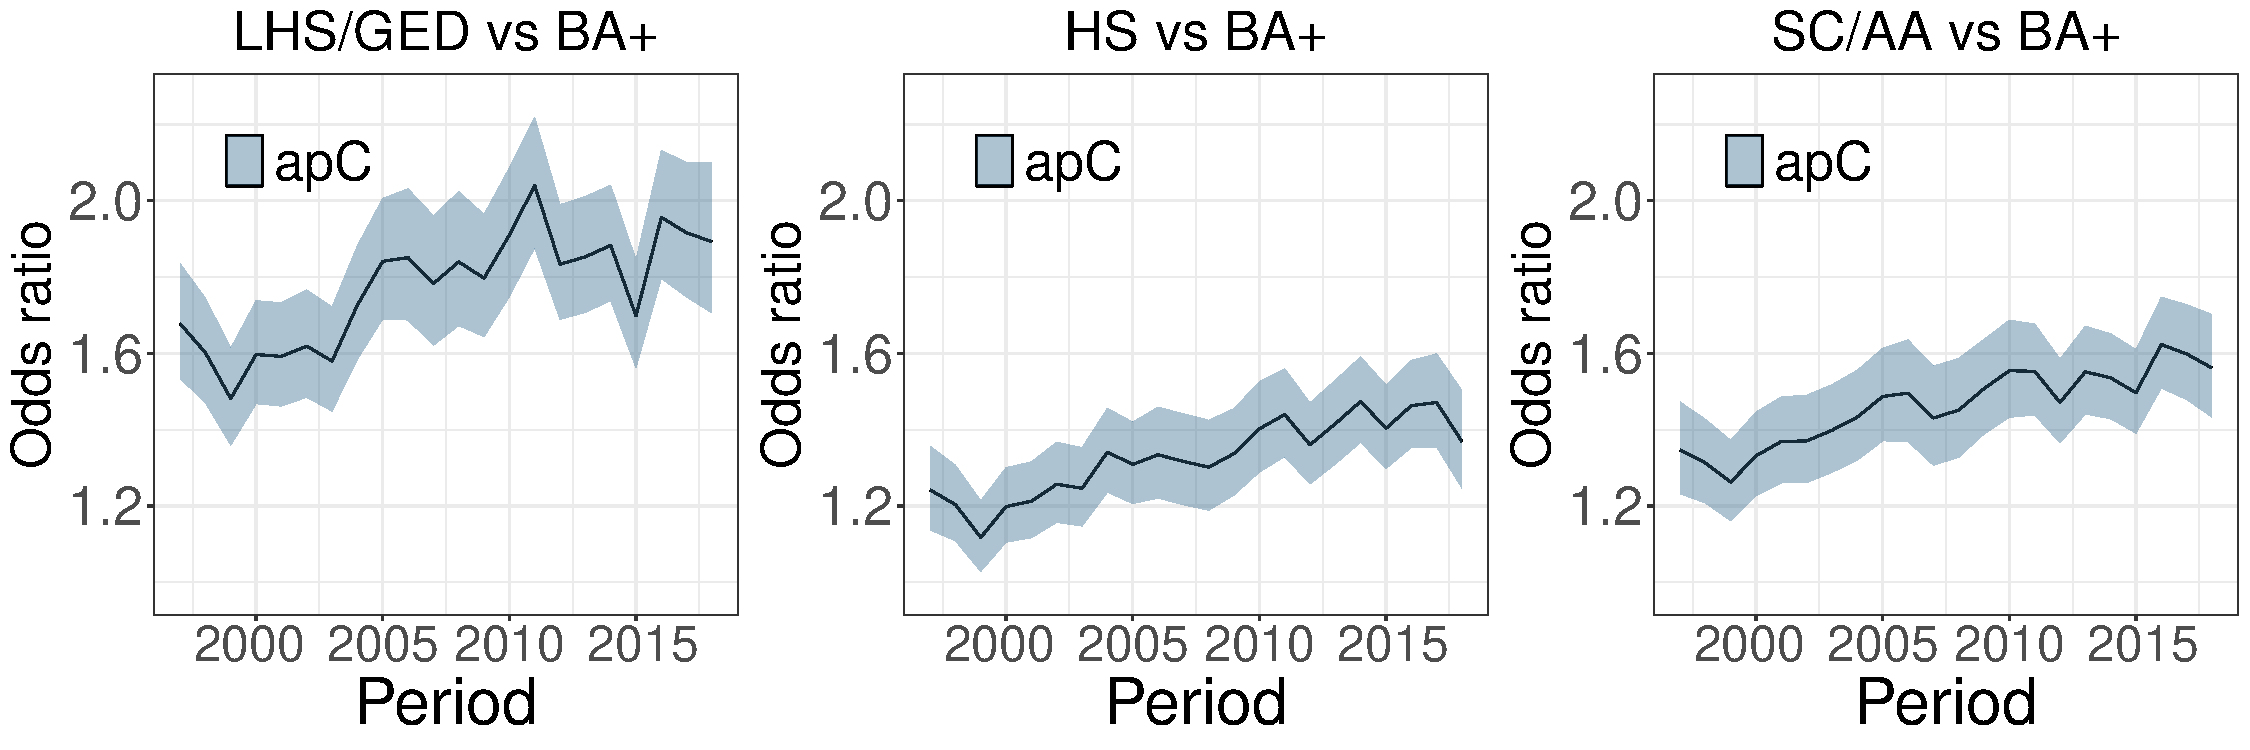
\includegraphics[width=\textwidth]{Figures/lincomb_period_f.pdf}
    \end{subfigure}
    \vskip\baselineskip\vspace{-0.3cm}
    \begin{subfigure}[b]{\textwidth}   
        \centering 
        \caption[]%
        {}    
        \label{figure:Application1:cohort_diff_f}
        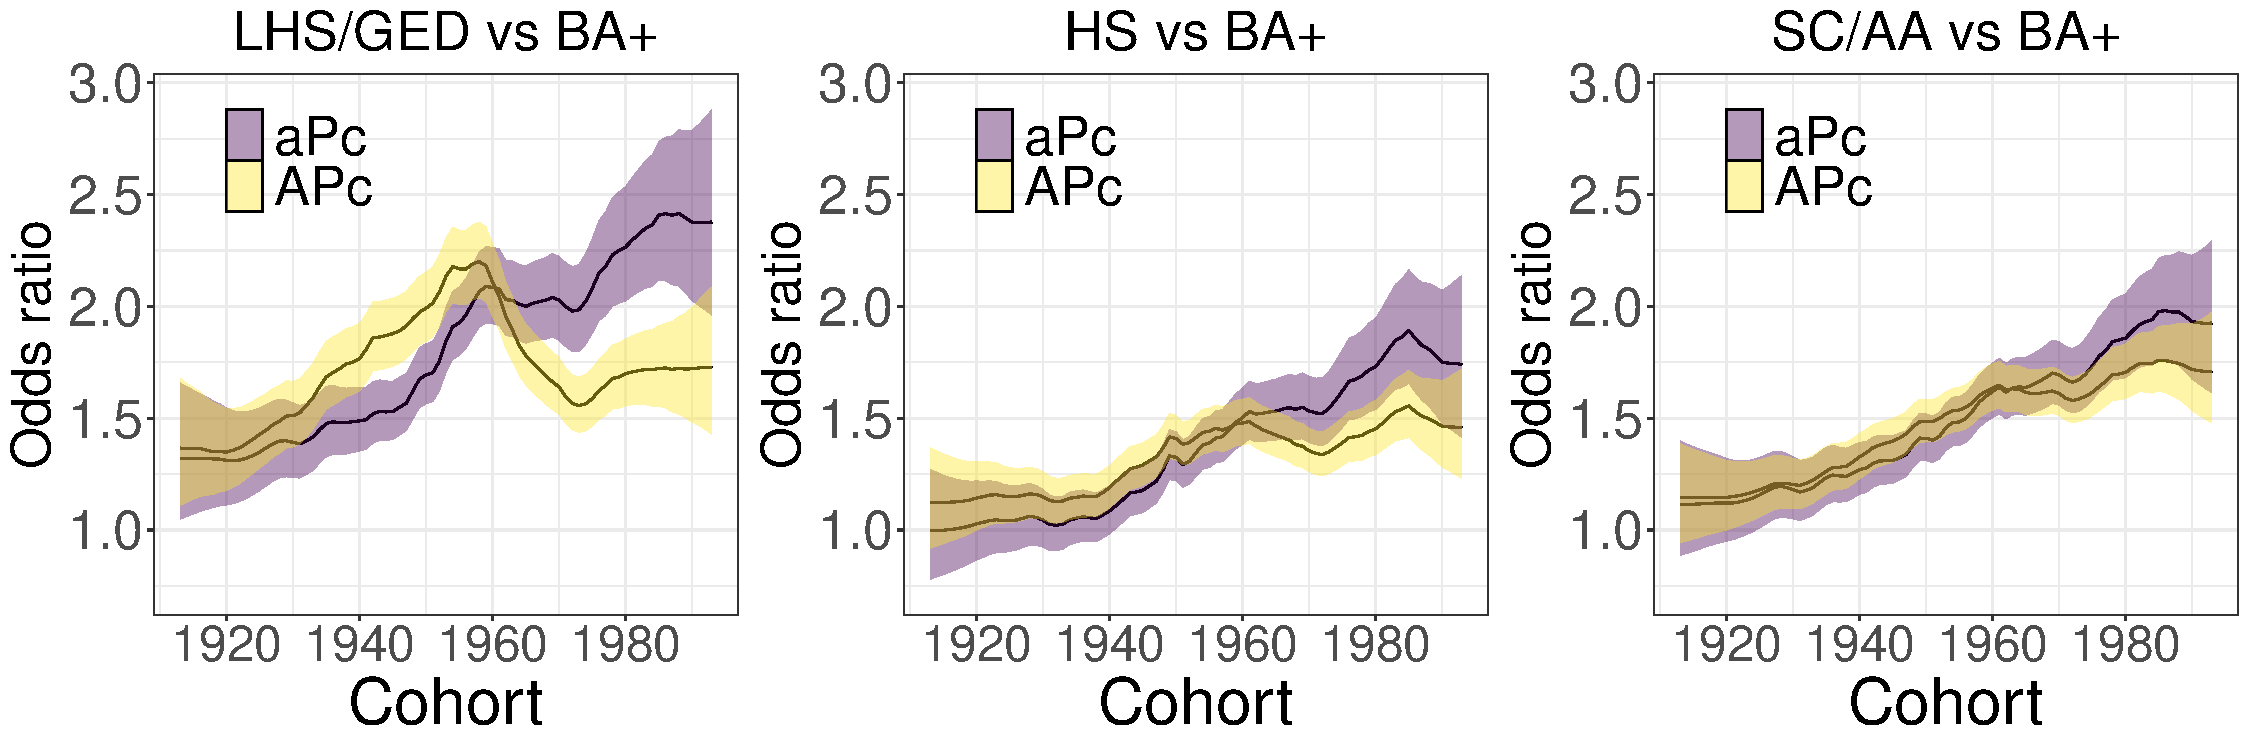
\includegraphics[width=\textwidth]{Figures/lincomb_cohort_f.pdf}
    \end{subfigure}
    \vspace{-0.3cm}
    \caption{For females with less than high school (LHS), high school (HS), and some college/associate of arts degree (SC/AA) levels of attained education with respect to bachelor or higher education, the posterior median odds ratio in the top four models by model selection over \textbf{(a)} age, \textbf{(b)} periods, and \textbf{(c)} cohorts, along with $95\%$ credible intervals.}
    \label{figure:Application1:lincombs_f}
\end{figure}

%Top3 models male
\begin{figure}
    \centering
    \begin{subfigure}[b]{\textwidth}   
        \centering 
        \caption[]%
        {}    
        \label{figure:Application1:age_diff_m}
        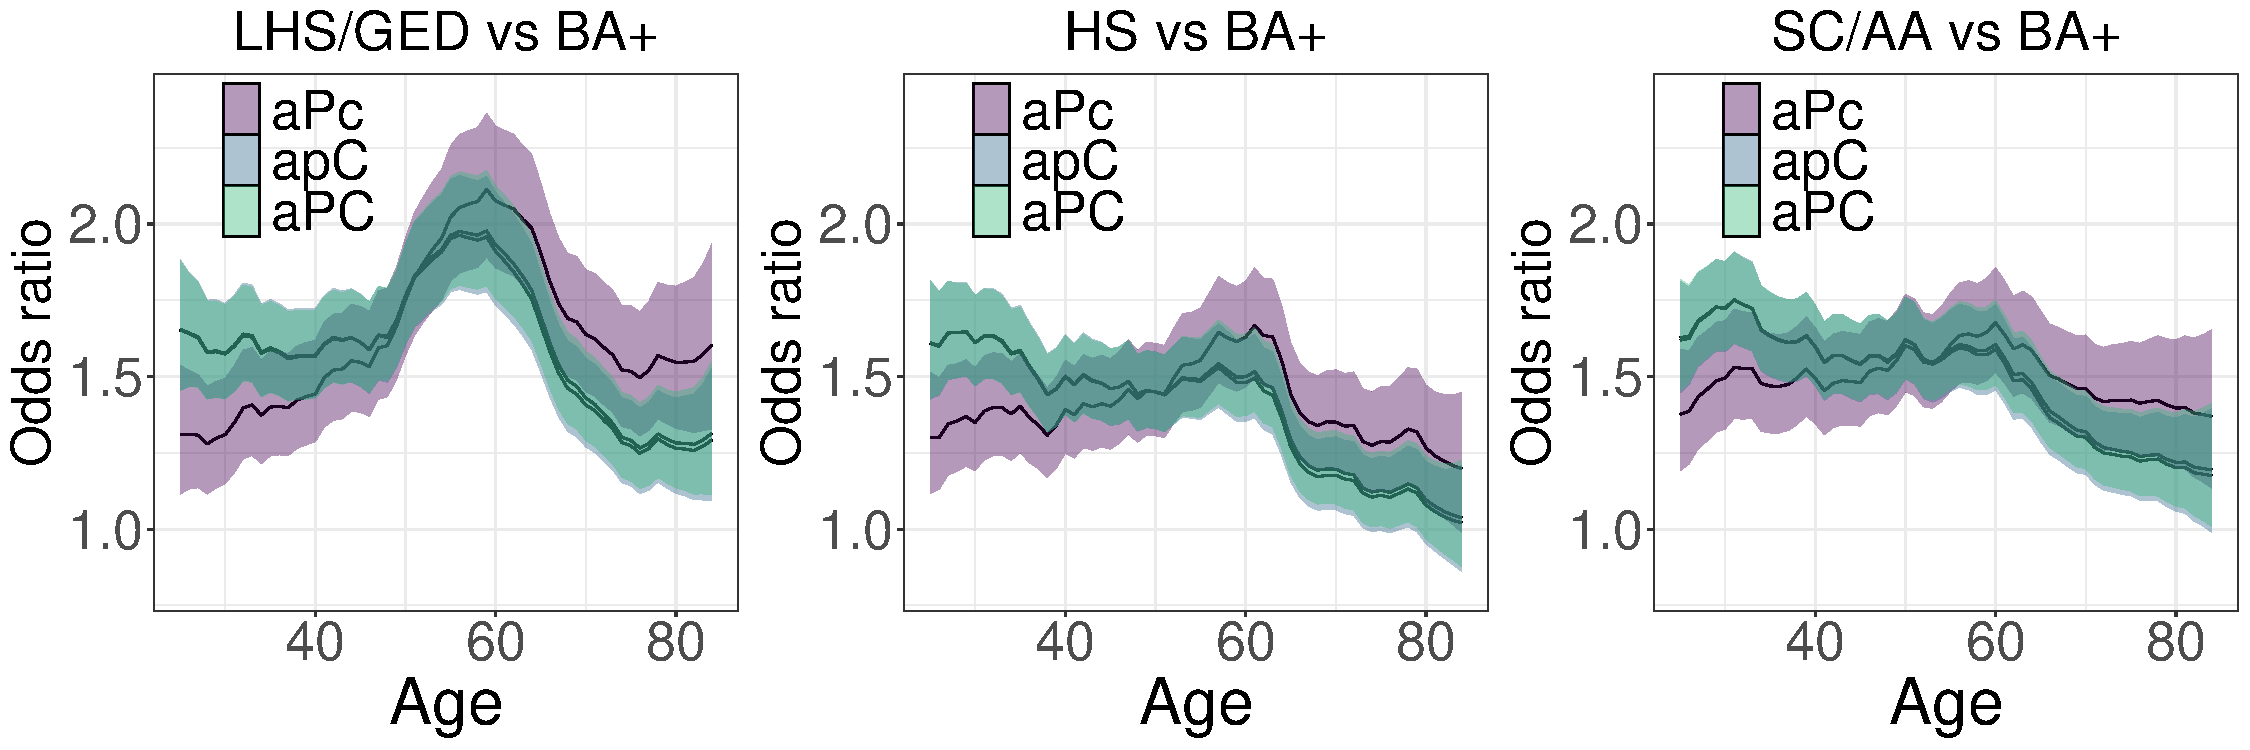
\includegraphics[width=\textwidth]{Figures/lincomb_age_m.pdf}
    \end{subfigure}
    \vskip\baselineskip\vspace{-0.3cm}
    \begin{subfigure}[b]{\textwidth}   
        \centering 
        \caption[]%
        {}    
        \label{figure:Application1:period_diff_m}
        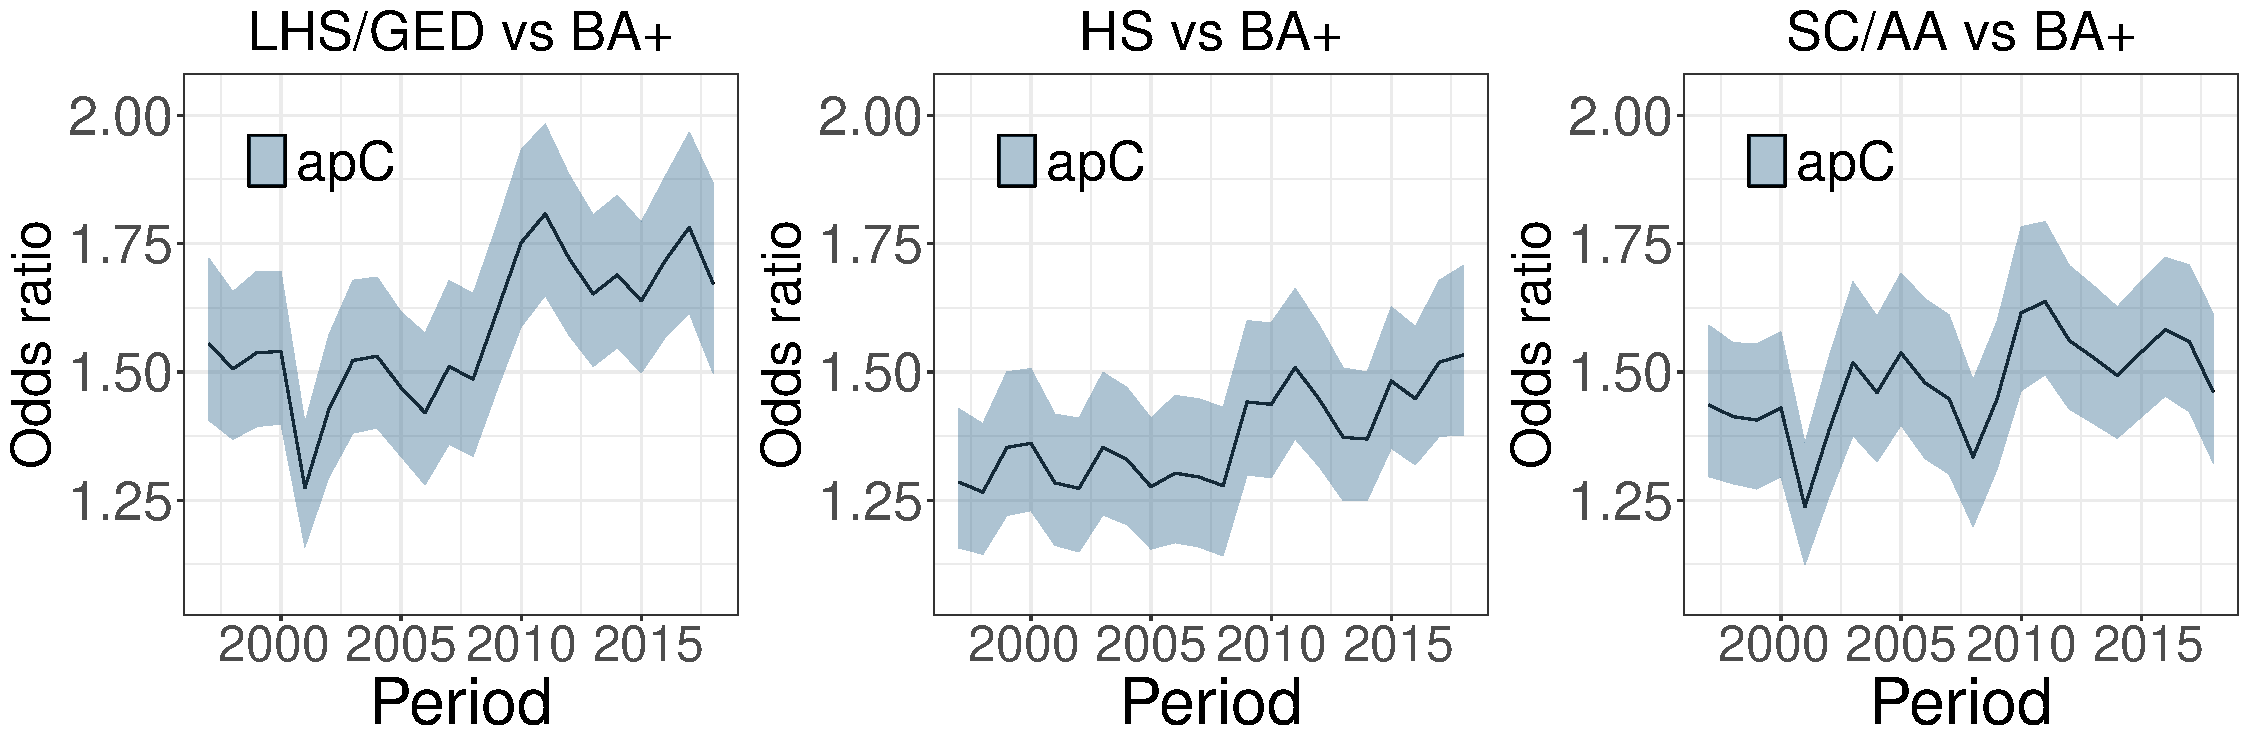
\includegraphics[width=\textwidth]{Figures/lincomb_period_m.pdf}
    \end{subfigure}
    \vskip\baselineskip\vspace{-0.3cm}
    \begin{subfigure}[b]{\textwidth}   
        \centering 
        \caption[]%
        {}    
        \label{figure:Application1:cohort_diff_m}
        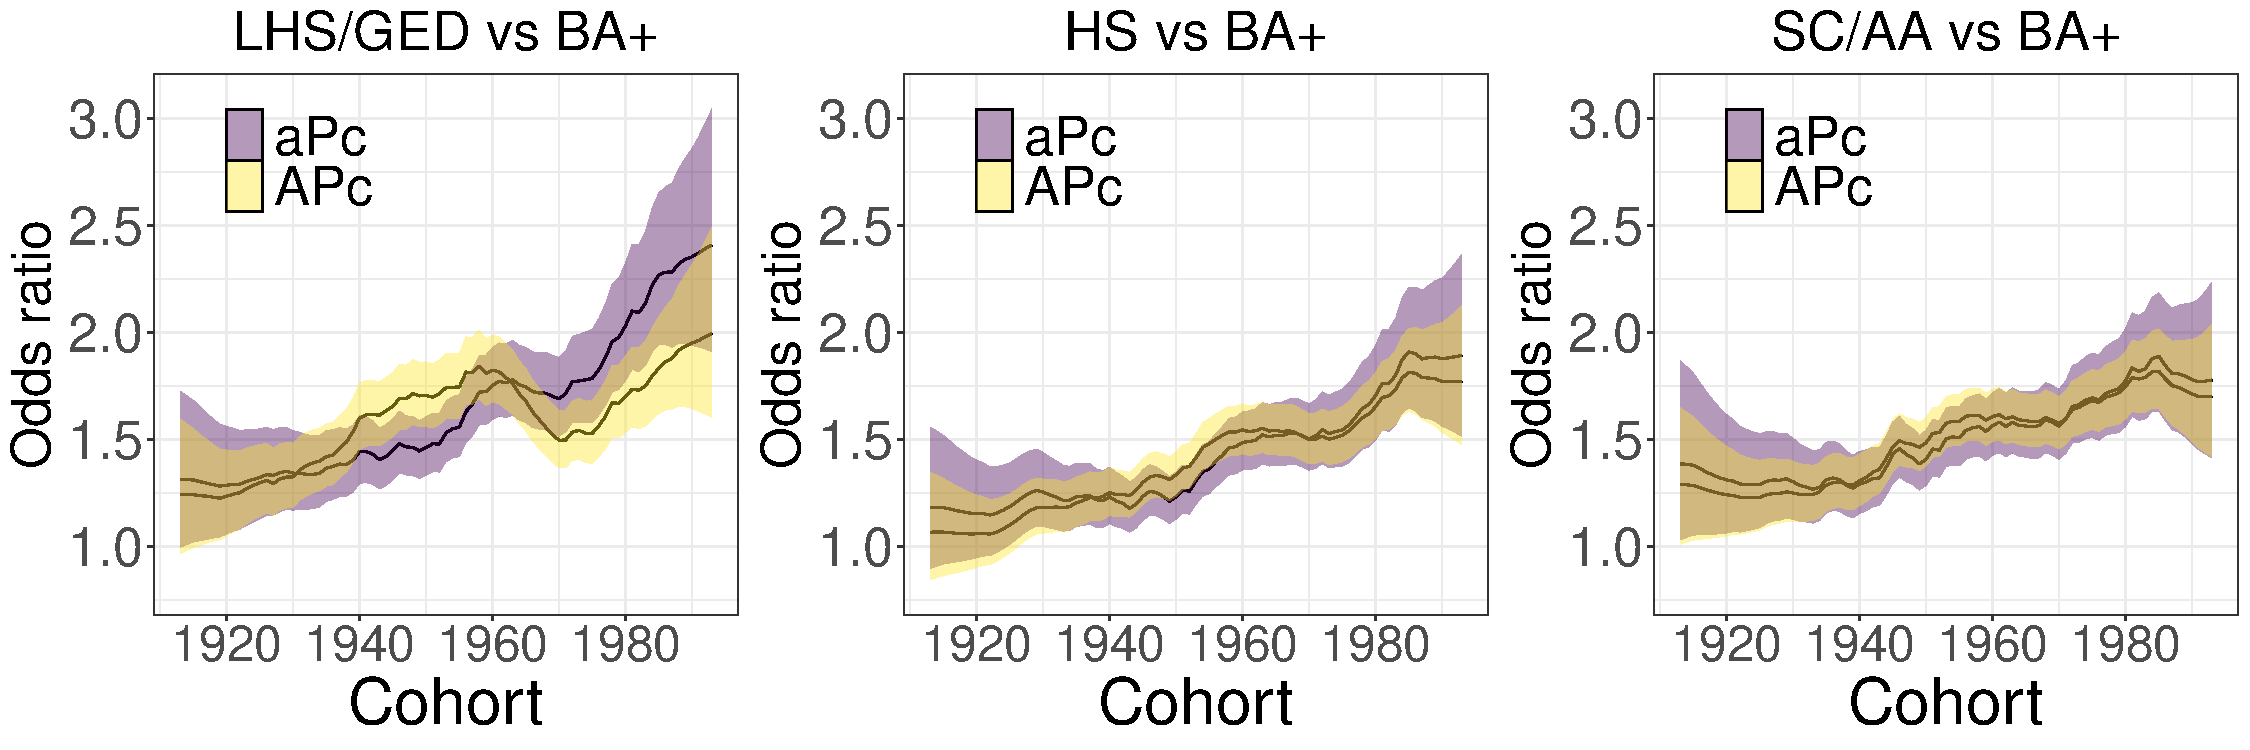
\includegraphics[width=\textwidth]{Figures/lincomb_cohort_m.pdf}
    \end{subfigure}
    \vspace{-0.3cm}
    \caption{For males with less than high school (LHS), high school (HS), and some college/associate of arts degree (SC/AA) levels of attained education with respect to bachelor or higher education, the posterior median odds ratio in the top four models by model selection over \textbf{(a)} age, \textbf{(b)} periods, and \textbf{(c)} cohorts, along with $95\%$ credible intervals.}
    \label{figure:Application1:lincombs_m}
\end{figure}

%Multiple models results
\subsubsubsection*{Top four models}
\vspace{-0.2cm}
The posterior medians of the odds ratio in the top four models chosen by model selection in Section \ref{section:model-selection} along with $95\%$ credible intervals are shown in Figure \ref{figure:Application1:lincombs_f} for female data and Figure \ref{figure:Application1:lincombs_m} for male data. Figures \ref{figure:Application1:age_diff_f} and \ref{figure:Application1:age_diff_m} show the estimated odds ratios over age in the aPc, apC, and aPC models. Over age, the estimated trends for the apC and aPC models are nearly identical, and are noticeably different from the trends estimated in the aPc model. As these are different models in terms of how the effects are modelled, some variation in the estimated trends is expected. It is interesting, however, to see that the model with stratum-specific cohort effects arrives at significantly different estimates than the models without. Meanwhile, due to the similar estimated trends in the apC and aPC models, it seems that stratification of the period effects cause little change in the estimates. Taken together, it seems that the combination of stratum-specific age and cohort effects is what affects the estimated trends the most. As for the odds ratio over period, in Figures \ref{figure:Application1:period_diff_f} and \ref{figure:Application1:period_diff_m}, we only have one model using a stratum-specific period effect (the apC model), meaning we have no models to compare the estimated trend with. Nevertheless, it is interesting to see that the estimated odds ratio trend over periods is generally slightly increasing with some fluctuation in all levels of attained education. Figures \ref{figure:Application1:cohort_diff_f} and \ref{figure:Application1:cohort_diff_m} show the estimated odds ratios over cohorts in the aPc and APc models. As we saw with these two models over age, the aPc and APc models arrive at noticeably different estimates of the odds ratios, particularly in LHS/GED level of attained education, where the odds ratios appear to decrease significantly between the $1960$ and $1970$ birth cohorts. This effect is quite drastic in the models using female data. Over the other levels of attained education, however, we see similar trends in both models for both sexes. Again, these differences indicate that different combinations of stratification by educational attainment in the age and cohort effects greatly influence the estimated trends, which underscores how crucial the age and cohort effects are when it comes to explaining the data.

\FloatBarrier
\subsection{Discussion}\label{section:Application1:Dicussion}
\subsubsubsection*{Summary}
\vspace{-0.2cm}
In this thesis so far, we have constructed a prior tailored for a Bayesian MAPC model, which incorporates provided sociological expert knowledge, as inspired by the approach used by \cite{IngeborgGenetics}, by using PC priors \citep{PC-priors}, together with the intuitive structure of HD priors \citep{Jointprior}. Moreover, the prior sensitivity analysis showed that the MAPC model in this application does not seem to be sensitive to the prior, since priors incorporating the "anti" expert knowledge showed similar results. From the model selection, models with different specifications of shared and stratum-specific age, period, and cohort effects were tested, and the model scores were found to be similar, though the aPc model appears to be slightly favored for both sexes. Then, interpreting the estimated cross strata differences in the aPc model as odds ratios (according to Section \ref{section:APC-inference}), the estimated odds ratios display clear temporal trends over age and cohorts. The estimated odds ratios among participants in all levels of attained education is generally increasing with age and more recent cohorts compared to that for the BA+ level, with substantially higher estimates among participants with the LHS/GED level of attained education. Consequently, our analysis shows rising differences in risk of back pain over age and cohorts, with some age groups and cohorts experiencing $2.5$ times as large odds of backpain as the corresponding group with BA+ level of attained education. Lastly, we examined the differences in the estimated trends between models using different combinations of shared and stratum-specific age, period, and cohort effects.

%Model selection, how robust
\subsubsubsection*{Model selection}
\vspace{-0.2cm}
The model selection performed in Section \ref{section:model-selection} revealed a preference for the aPc model in all scoring criteria when using male and female data separately. Interestingly, the computed logarithmic scores are very similar for all models, indicating that there is not a strong preference for any model overall. By looking at our secondary criteria, WAIC and DIC, we also see that there is a slight preference for the aPc model, though other models again achieve comparable scores. As a consequence, relying solely on the model scores for model selection is unadvised. Though in this case, the marginally better model happened to have education-specific age and cohort effects, which also were the effects indicated to have high importance by the EK. Therefore, this model naturally becomes the preferred model for further analysis in either case. As we saw with the prior sensitivity analysis, the posteriors did not change much when using different priors, meaning we would most likely still select the aPc model with a different prior specification. Slight variations in the data, on the other hand, could have resulted in a different preferred model due to the similarly achieved scores. 

%Shortly about GED disparity in general
\subsubsubsection*{Disparities in the LHS/GED educational group}
\vspace{-0.2cm}
In Section \ref{section:application1:results}, the estimated temporal trends in the aPc model revealed heterogeneous time trends across different levels of attained education for males and females separately. In both temporal trends, we observe rising differences compared to BA+ level of attained education, with estimates of the odds ratio greater than one almost everywhere. As discussed in Section \ref{section:APC-inference}, larger odds ratio indicates that the risk of back pain is heightened among participants with the given level of attained education, in comparison to the participants with BA+ level of attained education. Since this odds ratio is almost always greater than one, it indicates an overall disparity in health outcomes compared to BA+ level. In addition, we saw over both age and cohorts that participants with LHS/GED level of attained education is particularly at risk with larger estimated odds ratios than the corresponding age groups and cohorts with HS and SC/AA levels of attained education. This overall disparity compared to BA+ level, and particular disparity for the LHS/GED level of attained education has been observed already in other studies \citep{GEDdisparity}, which is reassuring and solidifies our grounds for temporal analysis and interpretation of the resulting trends.

%Age inverse V-shape
\subsubsubsection*{Trends over age}
\vspace{-0.2cm}
By our results, we elaborated upon these disparities in health by examining them in a temporal context, from which we observed similar trends over age in certain levels of attained education. In the models using male data, we saw an inverse V-shaped trend in all levels of attained education. The increasing risk of back pain with age makes sense since the age effect captures cumulative exposure to risk, as discussed in Section \ref{section:lexis}. What is interesting to see is that the risk of back pain appears to decrease noticeably compared to BA+ level after age $60$. The decrease could be attributed to multiple potential reasons, and the exact causes and explanations are better left to sociologist. However, one possible partial explanation could be due to selective mortality \citep{beckett2000converging, house1990age, lynch2003cohort}. The older age groups could consist of the survivors of their generation, meaning they are the ones of their generation who survived to old age. Thus, we only have observations on participants with exceptionally good health, since those with worse health may have already died before reaching old age. Thus, the health outcomes of these survivors may appear more in line with the health outcomes of participants with BA+ level of attained education. Therefore, the decrease could be, at least in part, due to higher mortality in the other levels of education compared to BA+ level. This could also be particularly the case for LHS/GED level of attained education, in which we observe the greatest decrease and disparities post age group $60$. Several factors are likely at play here, and further interpretation and investigation by experts would be beneficial in explaining the observed temporal trends.

%Difference between female and male estimates
\subsubsubsection*{Comparison between males and females}
\vspace{-0.2cm}
In our estimated trends, both similarities and differences were observed by sex. Over cohorts, the estimated trends are very similar in shape and magnitude, though for participants with LHS/GED level of attained education, we observe higher estimates for males than females between the $1940$ and $1980$ birth cohorts. Overall, these trends over cohorts are very similar in both sexes, indicating a similar evolution of socioeconomic factors over cohorts for both sexes, within all levels of attained education. Over age, substantially higher risk was observed among females compared to males with LHS/GED level of attained education. Moreover, the estimated trends were quite different for HS level of attained education. In females, we saw an increasing trend between ages $25$ to $50$, after which it became stagnant, while for males we observe an increasing trend until age $60$, after which it declines. The exact causes of these observed differences, particularly for the younger ages, are difficult to gauge at, and once again calls for sociologists to interpret.

%Alternative models results
\subsubsubsection*{Trends in alternative models}
\vspace{-0.2cm}
When considering the alternative, similar scoring models to the aPc models, we saw that the estimated trends over both age and cohorts differ noticeably depending on what effects are stratified by educational attainment. Interestingly, in alternative models to the aPc model, we still observe the inverse V-shape trend over age, though with an even more significant decrease in risk after age $60$. Interestingly, the two different trends in each group of education over age appear to be rotations of each other. However, this is not a cause for concern, as the models are inherently distinct from each other due to the different specifications of shared and stratum-specific effects. Moreover, over cohorts with LHS/GED level of attained education, we observe strange behaviors in the alternative model with a sudden dip in risk between the $1960$ and $1970$ birth cohort, in particular for females. While we see differences in the estimated trends over cohorts for all levels of education, none of them are as great and as abrupt as for LHS/GED level of attained education, calling for further investigation on the trends for this level of attained education. In all models, the estimated odds ratios are still greater than one everywhere, meaning that the overall disparity in health for all levels of attained education compared to BA+ level remains readily apparent. Coupled with the small differences in model scores, great care should be taken when selecting a model to analyse, and the context of which effects are stratified by education should be taken into account in the interpretation. 

%Prior sensitivity results
\subsubsubsection*{Prior sensitivity}
\vspace{-0.2cm}
From the prior sensitivity analysis in Section \ref{section:application1:prior-sens-result}, the aPc model chosen by model selection shows remarkable similarities when fitted with different priors. The models largely gravitate towards placing the posterior mass of the weight parameters in the same vicinity, meaning that the models do not appear to be sensitive to the prior. Moreover, the models distribute most of the variance to the age and cohort effects, which also happen to be the stratum-specific effects, which underscores the importance of the effects and stratification by educational attainment. Interestingly, the structured effects given large weight by the expert knowledge are also given large weight in the posterior in all models despite the different priors, which shows that the attribution of variance among the structured effects in the EK was appropriate. Despite induced shrinkage to the unstructured effect, the variance attributed to this effect was very small, and nearly all the variance was explained by the structured effects. The shrinkage was induced in the model to avoid overfitting, so the large attribution of variance to the structured effects indicates that the data is highly informative in the model fit. While a more formal approach could be preferred in prior sensitivity analysis, the approach used here proved sufficient for the application.

%Overall conclusions
\subsubsubsection*{Conclusion}
\vspace{-0.2cm}
Overall, our temporal analysis has provided clear evidence of disparities in risk of back pain based on educational attainment, and the estimated temporal trends displayed interesting patterns to be interpreted by sociologists. Should health conditions such as chronic back pain serve as a good barometer for the general health of a population, then our temporal analysis on disparities in health should inspire further investigation and discussion on the topic. Moreover, in addition to the exaggerated risk of back pain observed for the LHS/GED level of attained education compared to the other educational attainment levels, we also observe strange behaviors across different MAPC models it this level of attained education. Coupled with the already exaggerated risk of this group, and lower sample sizes in the survey data (as seen in Section \ref{section:data:explorative}), further investigations are needed to answer questions regarding participants with LHS/GED level of attained education. We have yet to account for the sampling design of the NHIS, which may provide new insights into our observations on the effects of education on back pain.

